\chapter{Results}

This chapter is divided into three sections. In the first section performances of the SARSA($\lambda$) algorithm, with the configuration are analysed. For each function results obtained applying the four different declinations of {\tt SARSA($\lambda$)} algorithm are compared. Remember that the four possible declinations are :

\begin{itemize}
	\item Linear, not random search
	\item Linear, random search
	\item Parametric, not random search
	\item Parametric, random search
\end{itemize}

Evaluations are made only on the greedy episode. The reason for this choice is to consider the algorithm's performances after giving a good enough training space composed by $150$ episodes, each one of $101$ epochs. \\

Three different plots for three different metrics are employed. The first one measures the \textit{Euclidean distance} \footnote{In mathematics, the Euclidean distance is the "ordinary" straight-line distance between two points in an Euclidean space. It is computed as follow: 
	
	\begin{equation}
		Euclidean\_distance = \sqrt{(x\textsubscript{i+n} - x_i)^2 + (y\textsubscript{i+n} - y_i)^2}
	\end{equation}

with $n \ge 0$. \\
	
Note that this performance metric is evaluated on the true function values but this information is not available for the optimization methods.} between point $(x_i, y_i)$ at epoch $e_i$, $\forall i \in n$ where $n$ is the number of epochs of greedy episode, and point $(x^*, y^*)$ which is the maximum. The second metric measures the \textit{function proximity in percentage} \footnote{The \textit{proximity in percentage} between the current value function and the optimal one is computed as follow:

\begin{equation}
Proximity\_in\_ percentage = \frac{currentValueFunction \times 100}{optimalValueFunction}
\end{equation}

Note that this performance metric is evaluated on the true function values but this information is not available to the optimization methods. \\ } between the current value function and the optimal one in the greedy episode. The third one represents the \textit{Gap metric}\footnote{This metric measures how effective each method is at finding the global maximum.

\begin{equation}
G_t = \dfrac{f(x^+, y^+) - f(x_1, y_1)}{f(x^* y^*) - f(x_1, y_1)}
\end{equation}

Where $x^+$ is the incumbent or best function sample found up to epoch $e$. The gap $G_t$ will therefore be a number between $0$ (indicating no improvement over the initial sample) and $1$ (if the incumbent is the maximum). Note that this performance metric is evaluated on the true function values but this information is not available to the optimization methods.~\cite{Hoffman:2011:PAB:3020548.3020587}} computed on the greedy episode. \\

In the second section a second experiment conducted adopting an \textit{experienced} version of the SARSA($\lambda$) algorithm will be described. In this case the algorithm is trained on different functions and evaluations are made on the greedy episode of the Styblinski-Tang's Revised function, run only using \textit{experience} acquired on other functions with no specific training on the function itself. \\

In the third section results obtained from experiment conducted on humans will be analysed.

\section{Basic SARSA($\lambda$) Algorithm's Performances}

\begin{figure}[h!]
	\begin{center}
		\subfigure[]{%
			\label{fig:HimmelblauDifference}
			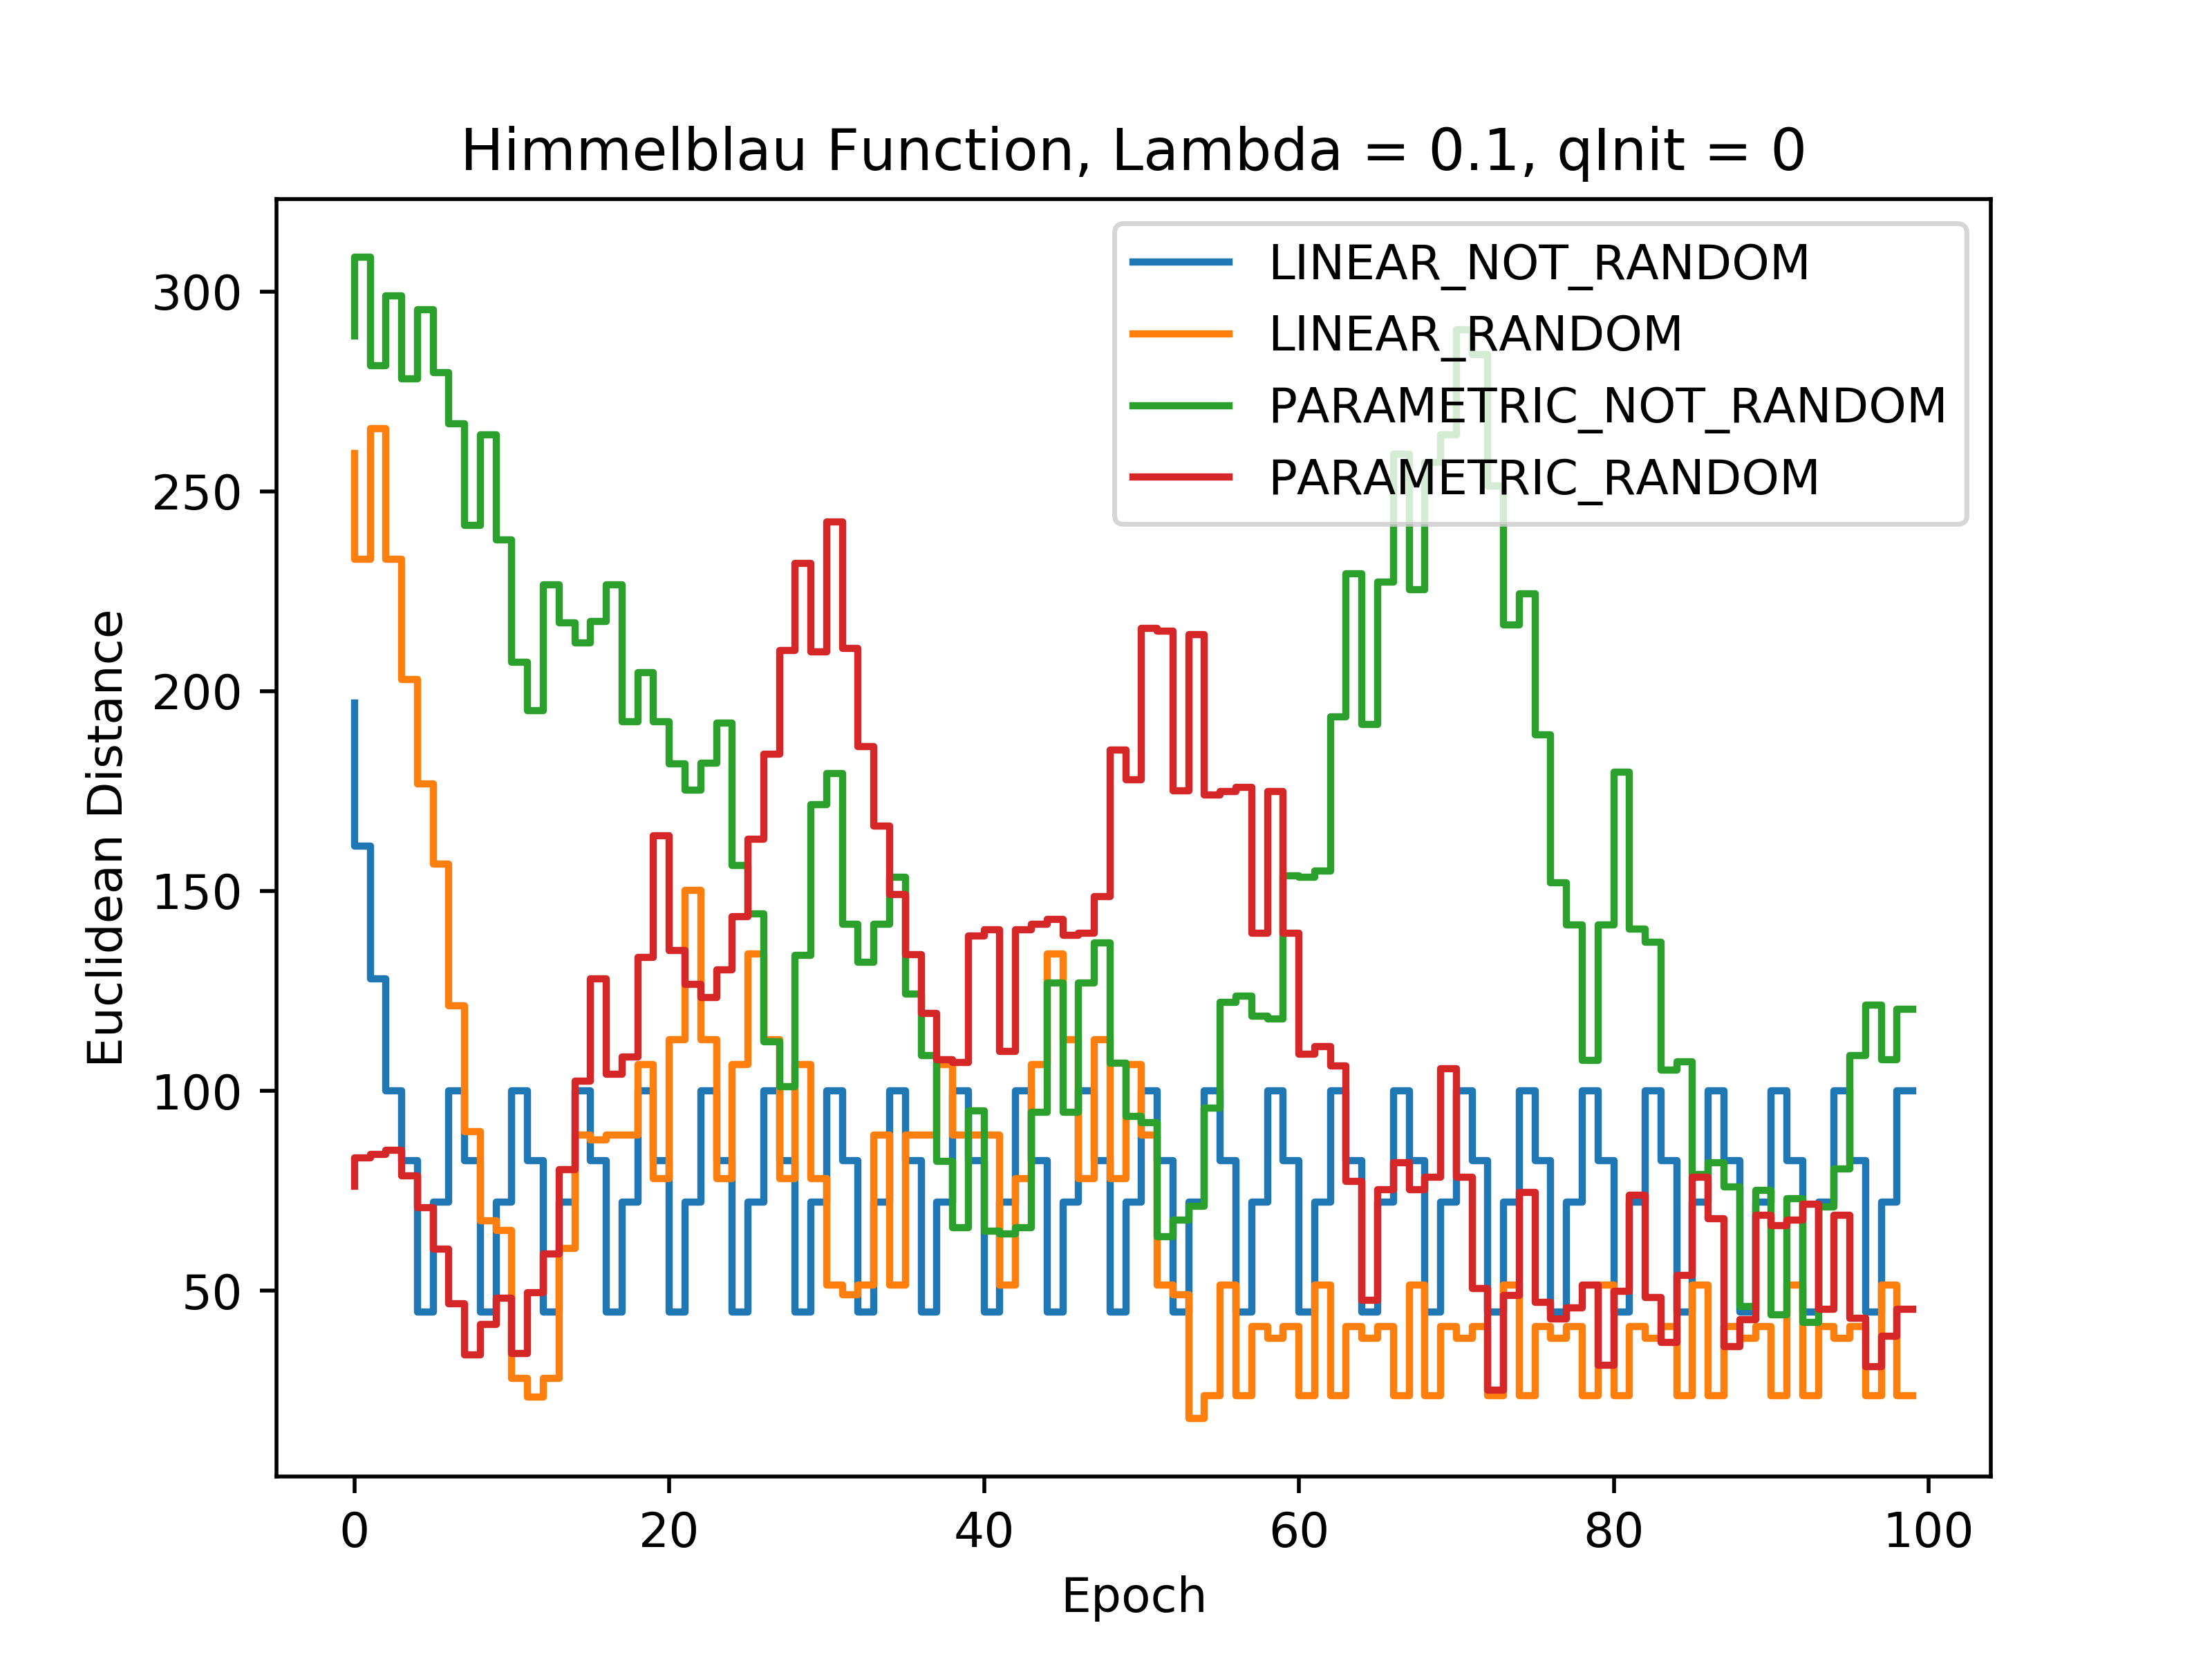
\includegraphics[width=0.4\textwidth]{HimmelblauDifference}
		}
		\subfigure[]{%
			\label{fig:HimmelblauValueFunction}
			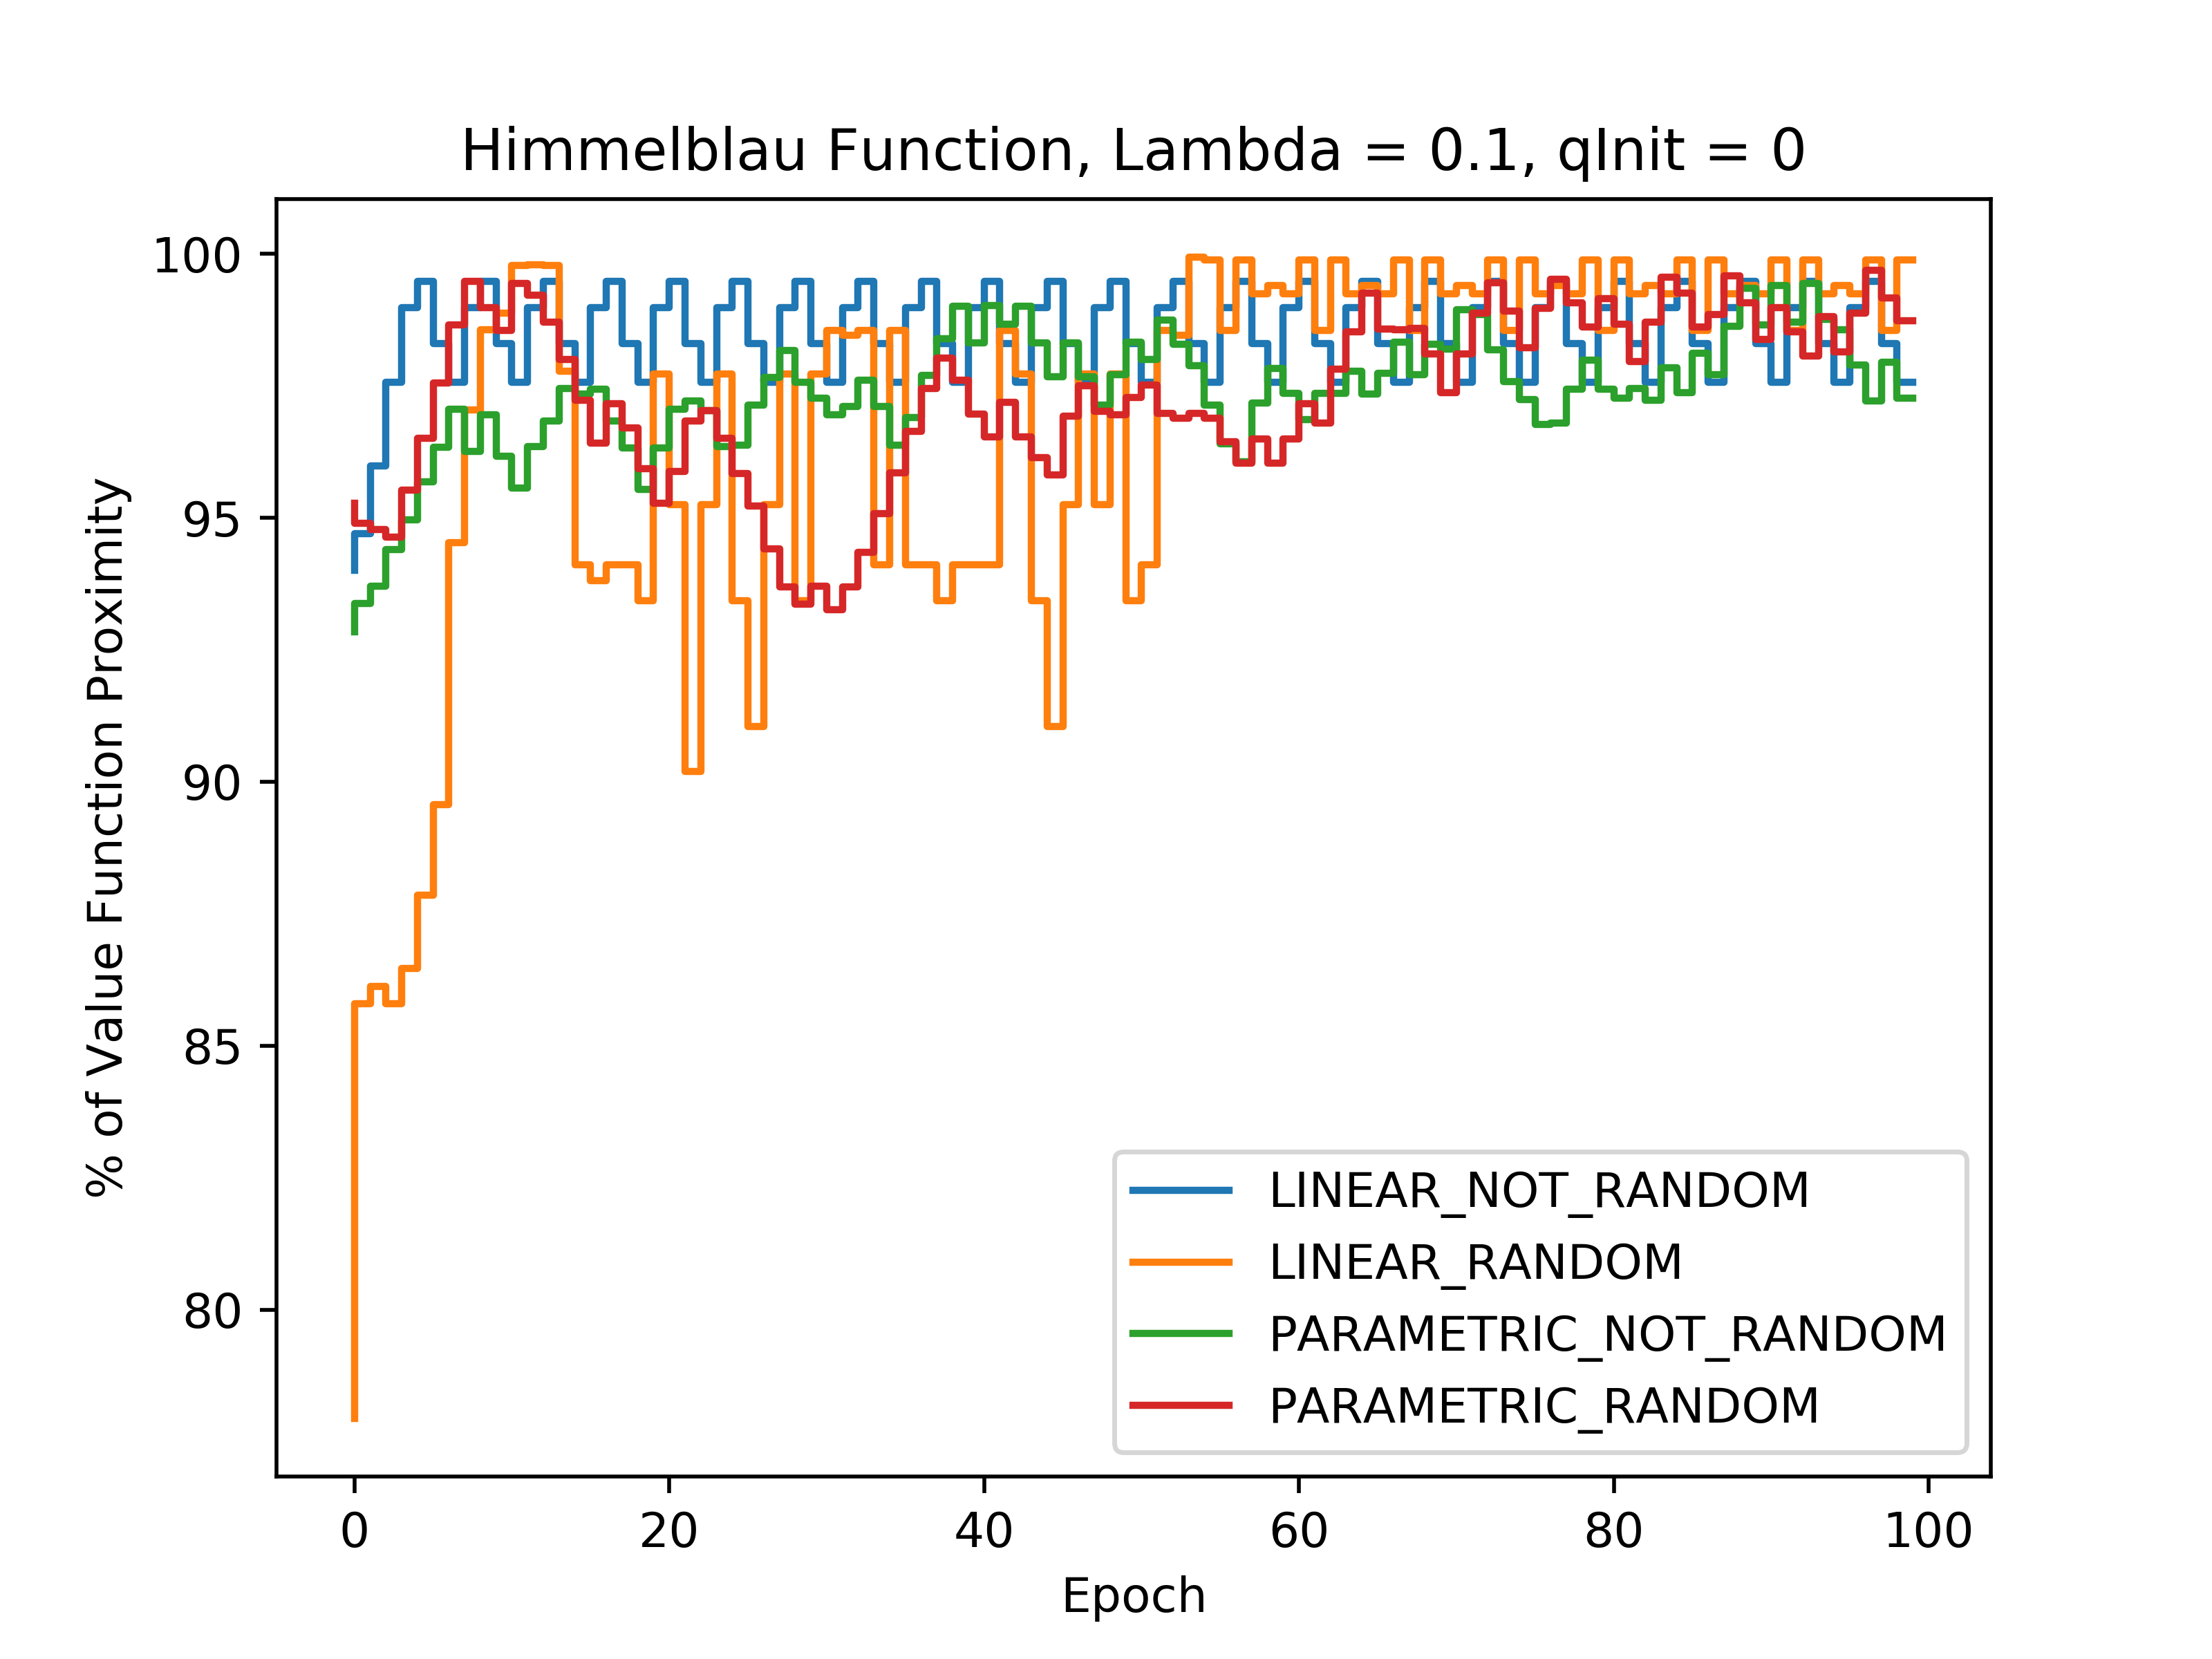
\includegraphics[width=0.4\textwidth]{HimmelblauValueFunction}
		}\\
		\subfigure[]{%
			\label{fig:HimmelblauGap}
			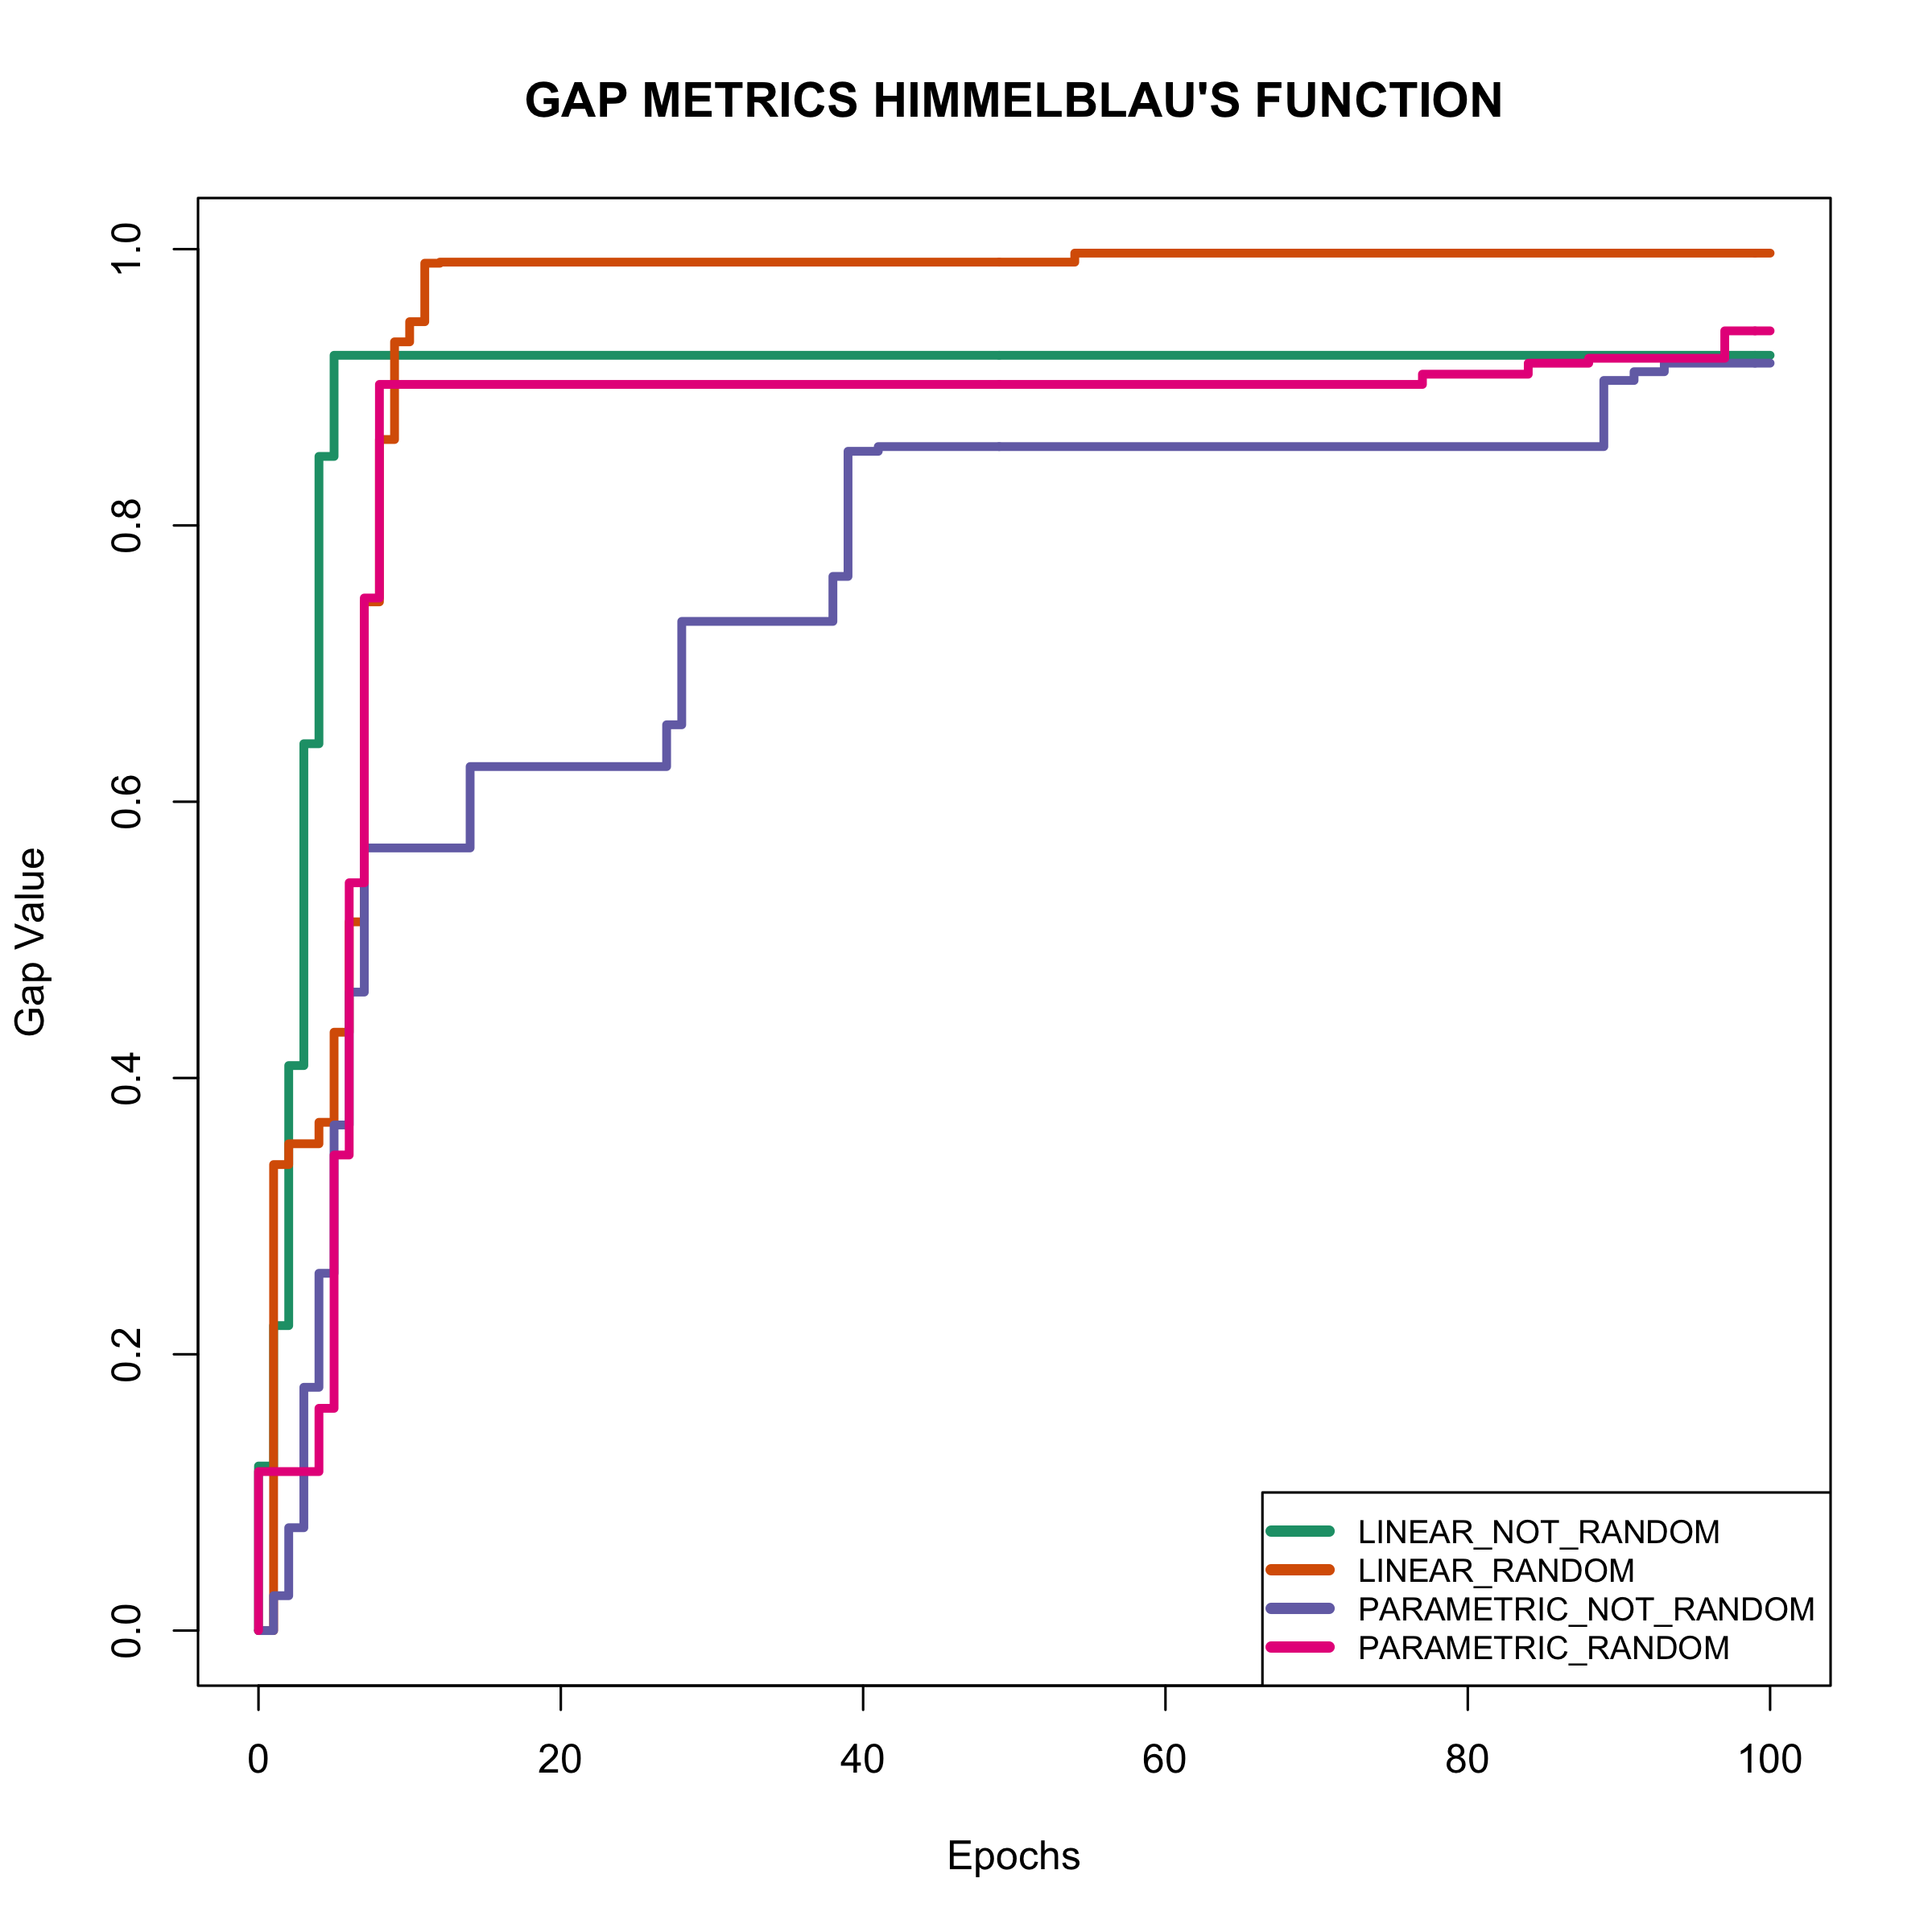
\includegraphics[width=0.4\textwidth]{HimmelblauGap}
		}		
	\end{center}
	\caption{
		Himmelblau' s Function.
	}
	\label{fig:HimmelblauResults}
\end{figure}

\subsection{Himmelblau' s Function} Plot (a) of figure \ref{fig:HimmelblauResults} graphically represents performances of the four possible declinations of {\tt SARSA($\lambda$)} algorithm obtained considering the \textit{Euclidean distance metric}. 

Looking at the {\tt linear, not random} declination's performance, it can be possible to note a starting high Euclidean difference between the agent's position and the global maximum. It decreases until epoch $5$. Starting from this epoch, a recurrent pattern starts to be developed. This behaviour depends on the fact that once the agent has achieved a good position compared to the maximum, it has to continue to make movements until the terminal state is achieved. Each movement implies a reward. The agent selects a set of movements that maximizes the reward and systematically repeats them. The stability just described is also proved by the fact that the standard deviation of the current declination is the lowest of the set with a value of $25.3$ (table $5.1$).

{\tt Linear, random} declination has a greater instability compared to the {\tt linear, not random} one. In the first fifty epochs the \textit{Euclidean distance} from the global maximum is constantly higher but then it starts to stabilize. Starting from the fiftieth epoch it develops a recurrent pattern and achieves best results. With an Euclidean distance mean of $71.6$ pixels from the maximum, it has the best performance of the set (table $5.1$).

The {\tt parametric, not random} declination has worst performances of the declinations' set. It is unable to minimize the Euclidean distance from the global maximum and it is highly unstable. Looking at table $5.1$ it is possible to note that the current declination as highest values in all statistic measures.

Finally, the {\tt parametric, random} declination selects a starting point near to the global maximum but it is unable to maintain a low Euclidean distance from it until epoch seventy. Starting from this epoch it develops a recurrent pattern similar to one previously described. Despite of this it is possible to say that its performances are worse compared to the first two ones.

Slower convergence of linear declinations compared to parametric ones depends on the fact that in the first case, as already explained in \textbf{Chapter $3$}, greater movements are done at each epoch and a lower training time is required to achieve the maximum. The amount of parametric movements are strictly conditioned by the function's shape. If this represents an obstacle to a fast convergence, however it is an incentive to an higher precision. \\

\begin{table} [h!]
	\centering
	\resizebox{\linewidth}{!} {
	\begin{tabular}{c| cccccc}
		\hline \textbf{Himmelblau' s Function}
		& \textbf{Mean (pixels)} & \textbf{Standard deviation}  \\ 
		\hline Linear not Random
		& $77.7$ &\cellcolor{red!25}$25.3$ \\ 
		\hline Linear Random
		& \cellcolor{red!25}$71.6$ & $52.2$ \\ 
		\hline Parametric not Random
		& $158.6$ & $71.3$ \\ 
		\hline Parametric Random
		& $105.5$ & $56.0$ \\ 
		\hline 
	\end{tabular}
}
\label{tab:HimmelblauTabEuclidean}
\caption{Euclidean Metric's Performances}
\end{table}

Plot (b) of figure ~\ref{fig:HimmelblauResults} graphically represents performances of the four possible declinations of {\tt SARSA($\lambda$)} algorithm obtained considering the \textit{Function Proximity in Percentage} metric.

All declinations, except for the {\tt linear, random} one, start with an high level of value function's proximity to the maximum. It depends on the function's shape. 

Once it has achieved a good enough proximal point to the maximum, the {\tt linear, not random} declination maintains always the same vale function's proximity level developing a recurrent pattern. The average level of proximity achieved by this declination is the best of the set (table $5.2$). The high stability of the current declination is proved by the lowest standard deviation of the set (table $5.2$). 

The {\tt linear, random} declination starts from a point not very close to the maximum in terms of value function's value. Its great instability reveals an inadequate training space. It starts to stabilize starting from the fiftieth epoch. Its starting instability is proved by the highest standard deviation of the set (table $5.2$).

The {\tt parametric, not random} declination reveals a general stability. The growth of proximity is slower then the corresponding linear declination because of the reduced amount of movement depending on the function's shape. 

Finally, the {\tt parametric, random} declination, as the corresponding linear declination, shows an initial instability. In general performances are more stable than the linear corresponding ones because of the lower amount of movement done at each epoch. Starting from the sixty-fifth epoch the proximity slowly grows and stabilizes. \\

\begin{table} [h!]
	\centering
	\resizebox{\linewidth}{!} {
	\begin{tabular}{c| cccccc} 
		\hline \textbf{Himmelblau' s Function}
		& \textbf{Mean (\%)} & \textbf{Standard deviation}  \\ 
		\hline Linear not Random
		& \cellcolor{green!25}$98.5$ & \cellcolor{green!25}$0.96$  \\ 
		\hline Linear Random
		& $96.8$ & $4.0$ \\ 
		\hline Parametric not Random
		& $97.4$ & $1.2$ \\ 
		\hline Parametric Random
		& $97.3$ & $1.6$ \\ 
		\hline 
	\end{tabular}
}
\label{HimmelblauTabProximity}
\caption{Function Proximity in Percentage.} 
\end{table}

Plot (c) of figure ~\ref{fig:HimmelblauResults} graphically represents performances of the four possible declinations of {\tt SARSA($\lambda$)} algorithm obtained considering the \textit{Gap metric}. According to this plot the most effective declination of {\tt SARSA($\lambda$)} algorithm in finding the maximum is the {\tt linear, random} one. Looking at table $5.9$ it is possible to note that {\tt linear, random} declination achieves point $(3.67, -1.57)$ with a value function of $2498.457$ out of $2500.0$.

\begin{figure}[h!]
	\begin{center}
		\subfigure[]{%
			\label{fig:ParabolicDifference}
			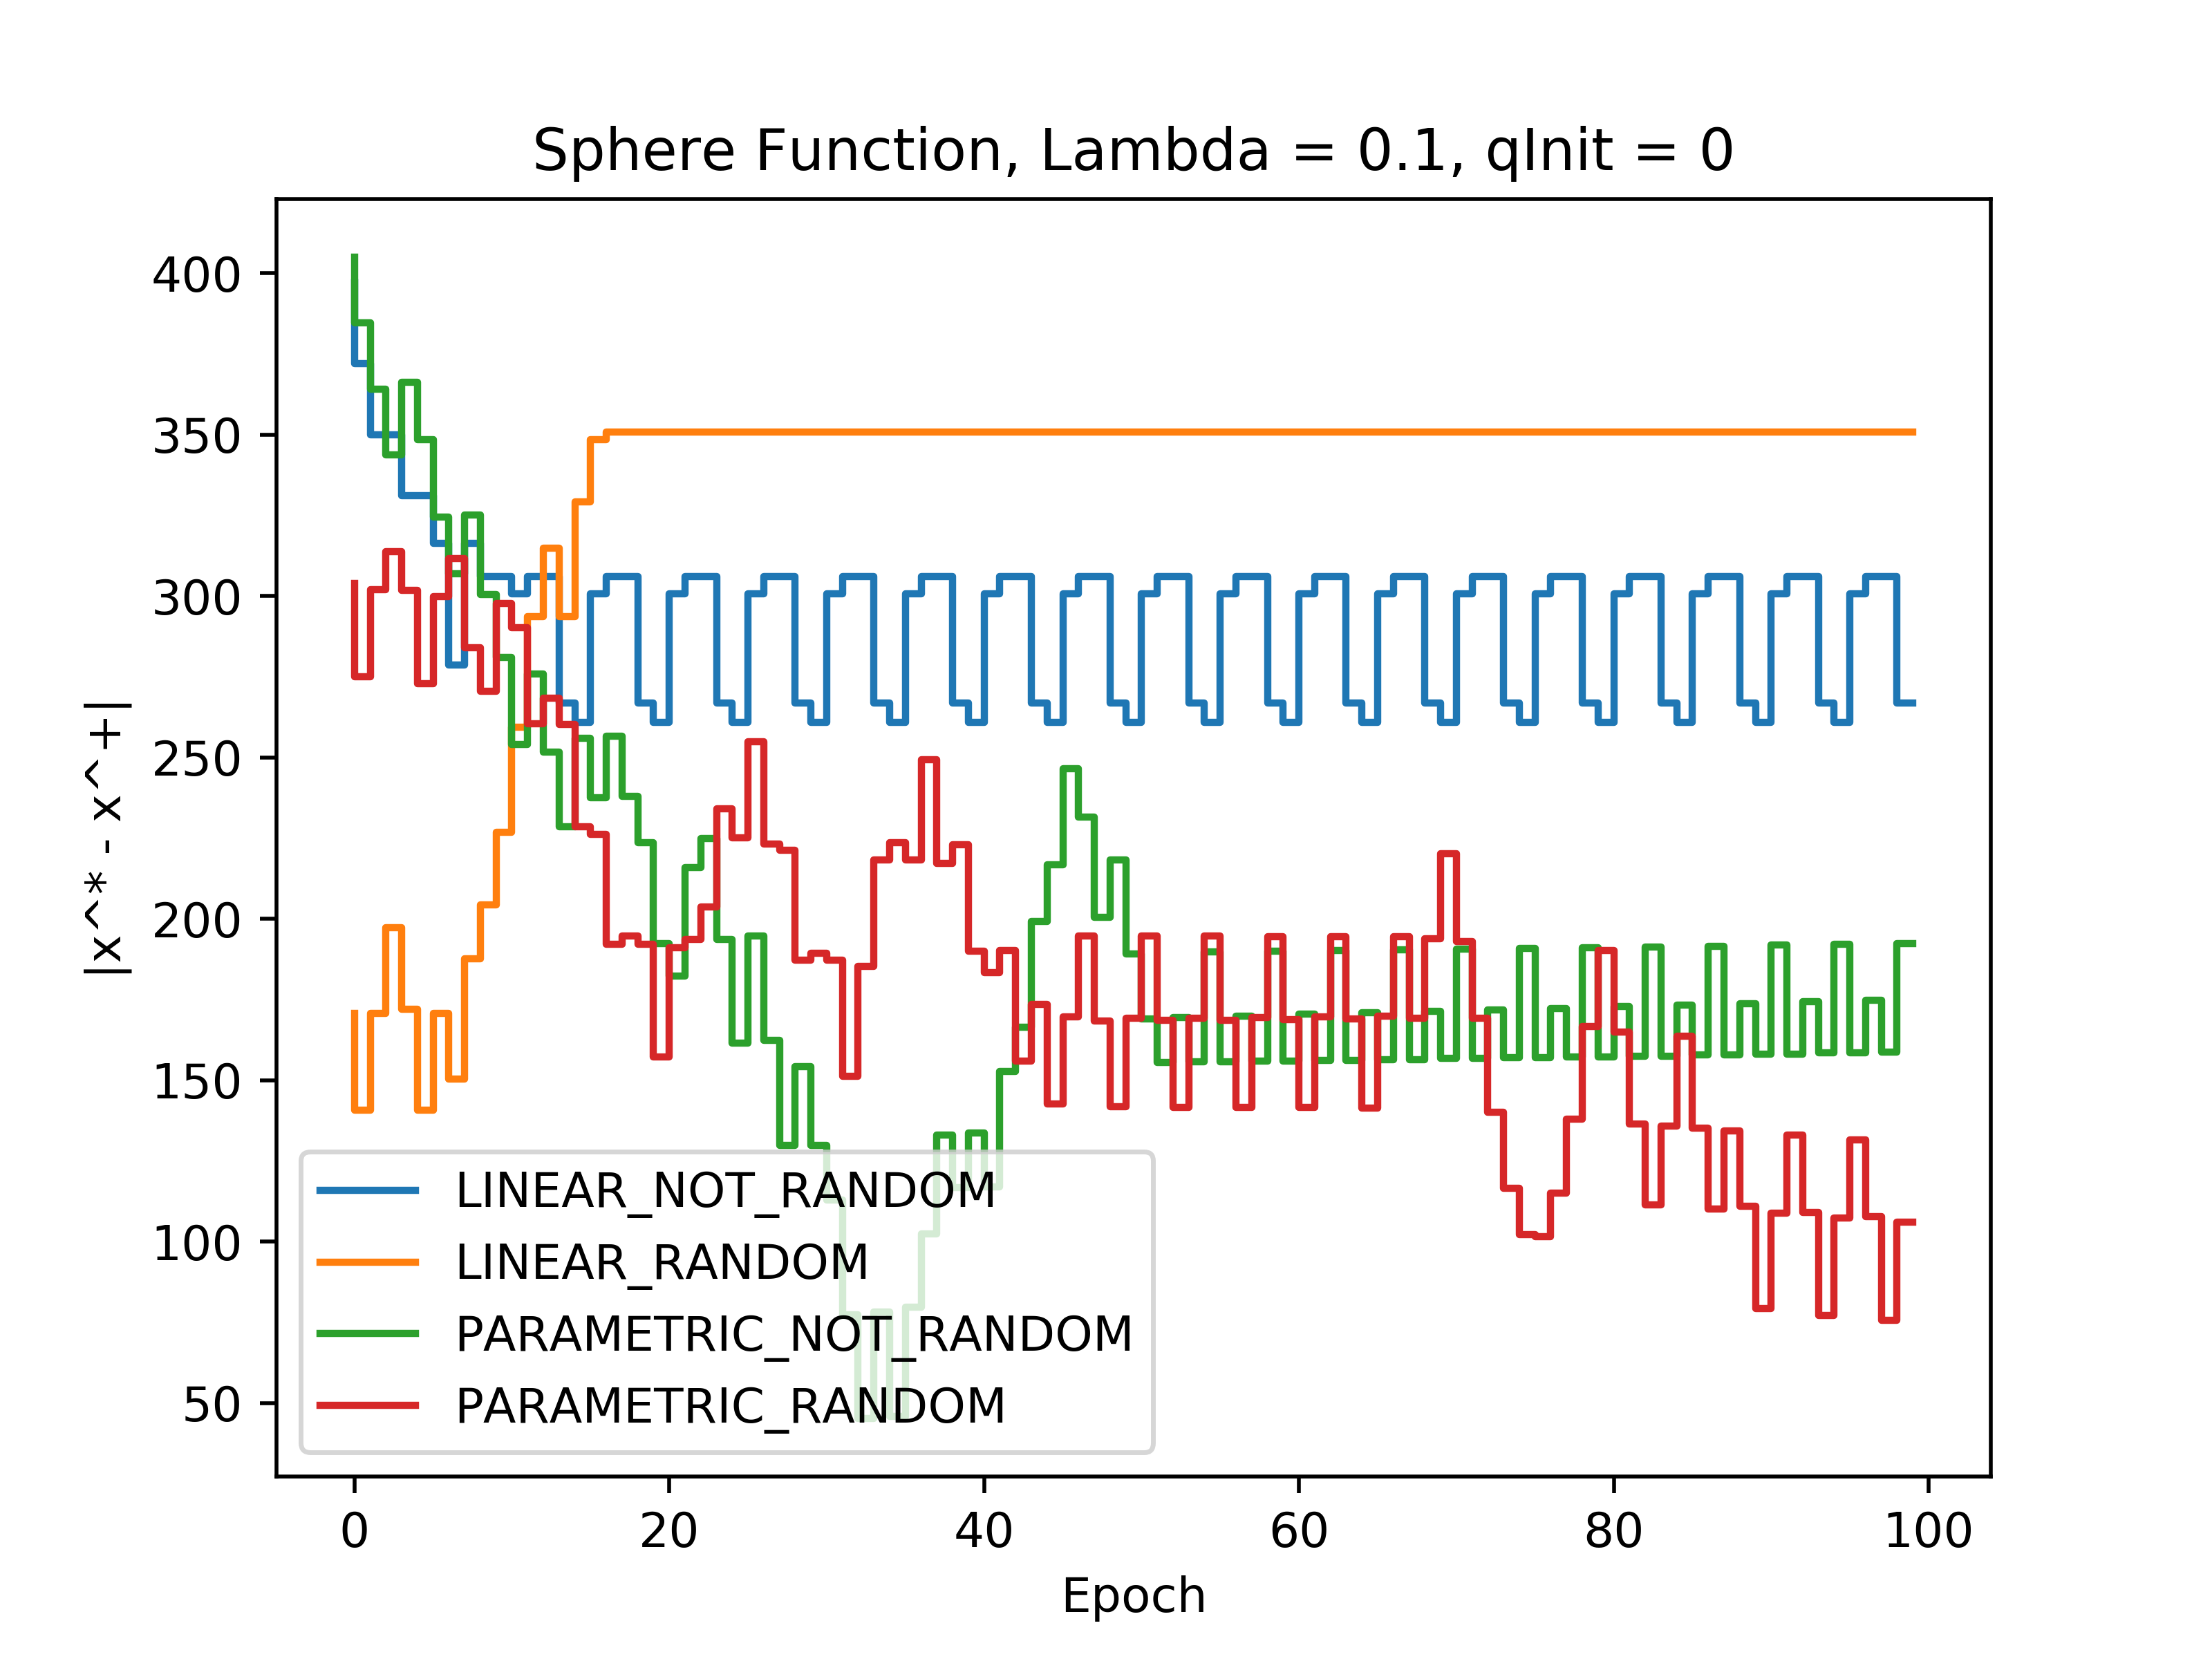
\includegraphics[width=0.4\textwidth]{ParabolicEuclidean}
		}
		\subfigure[]{%
			\label{fig:ParabolicValueFunction}
			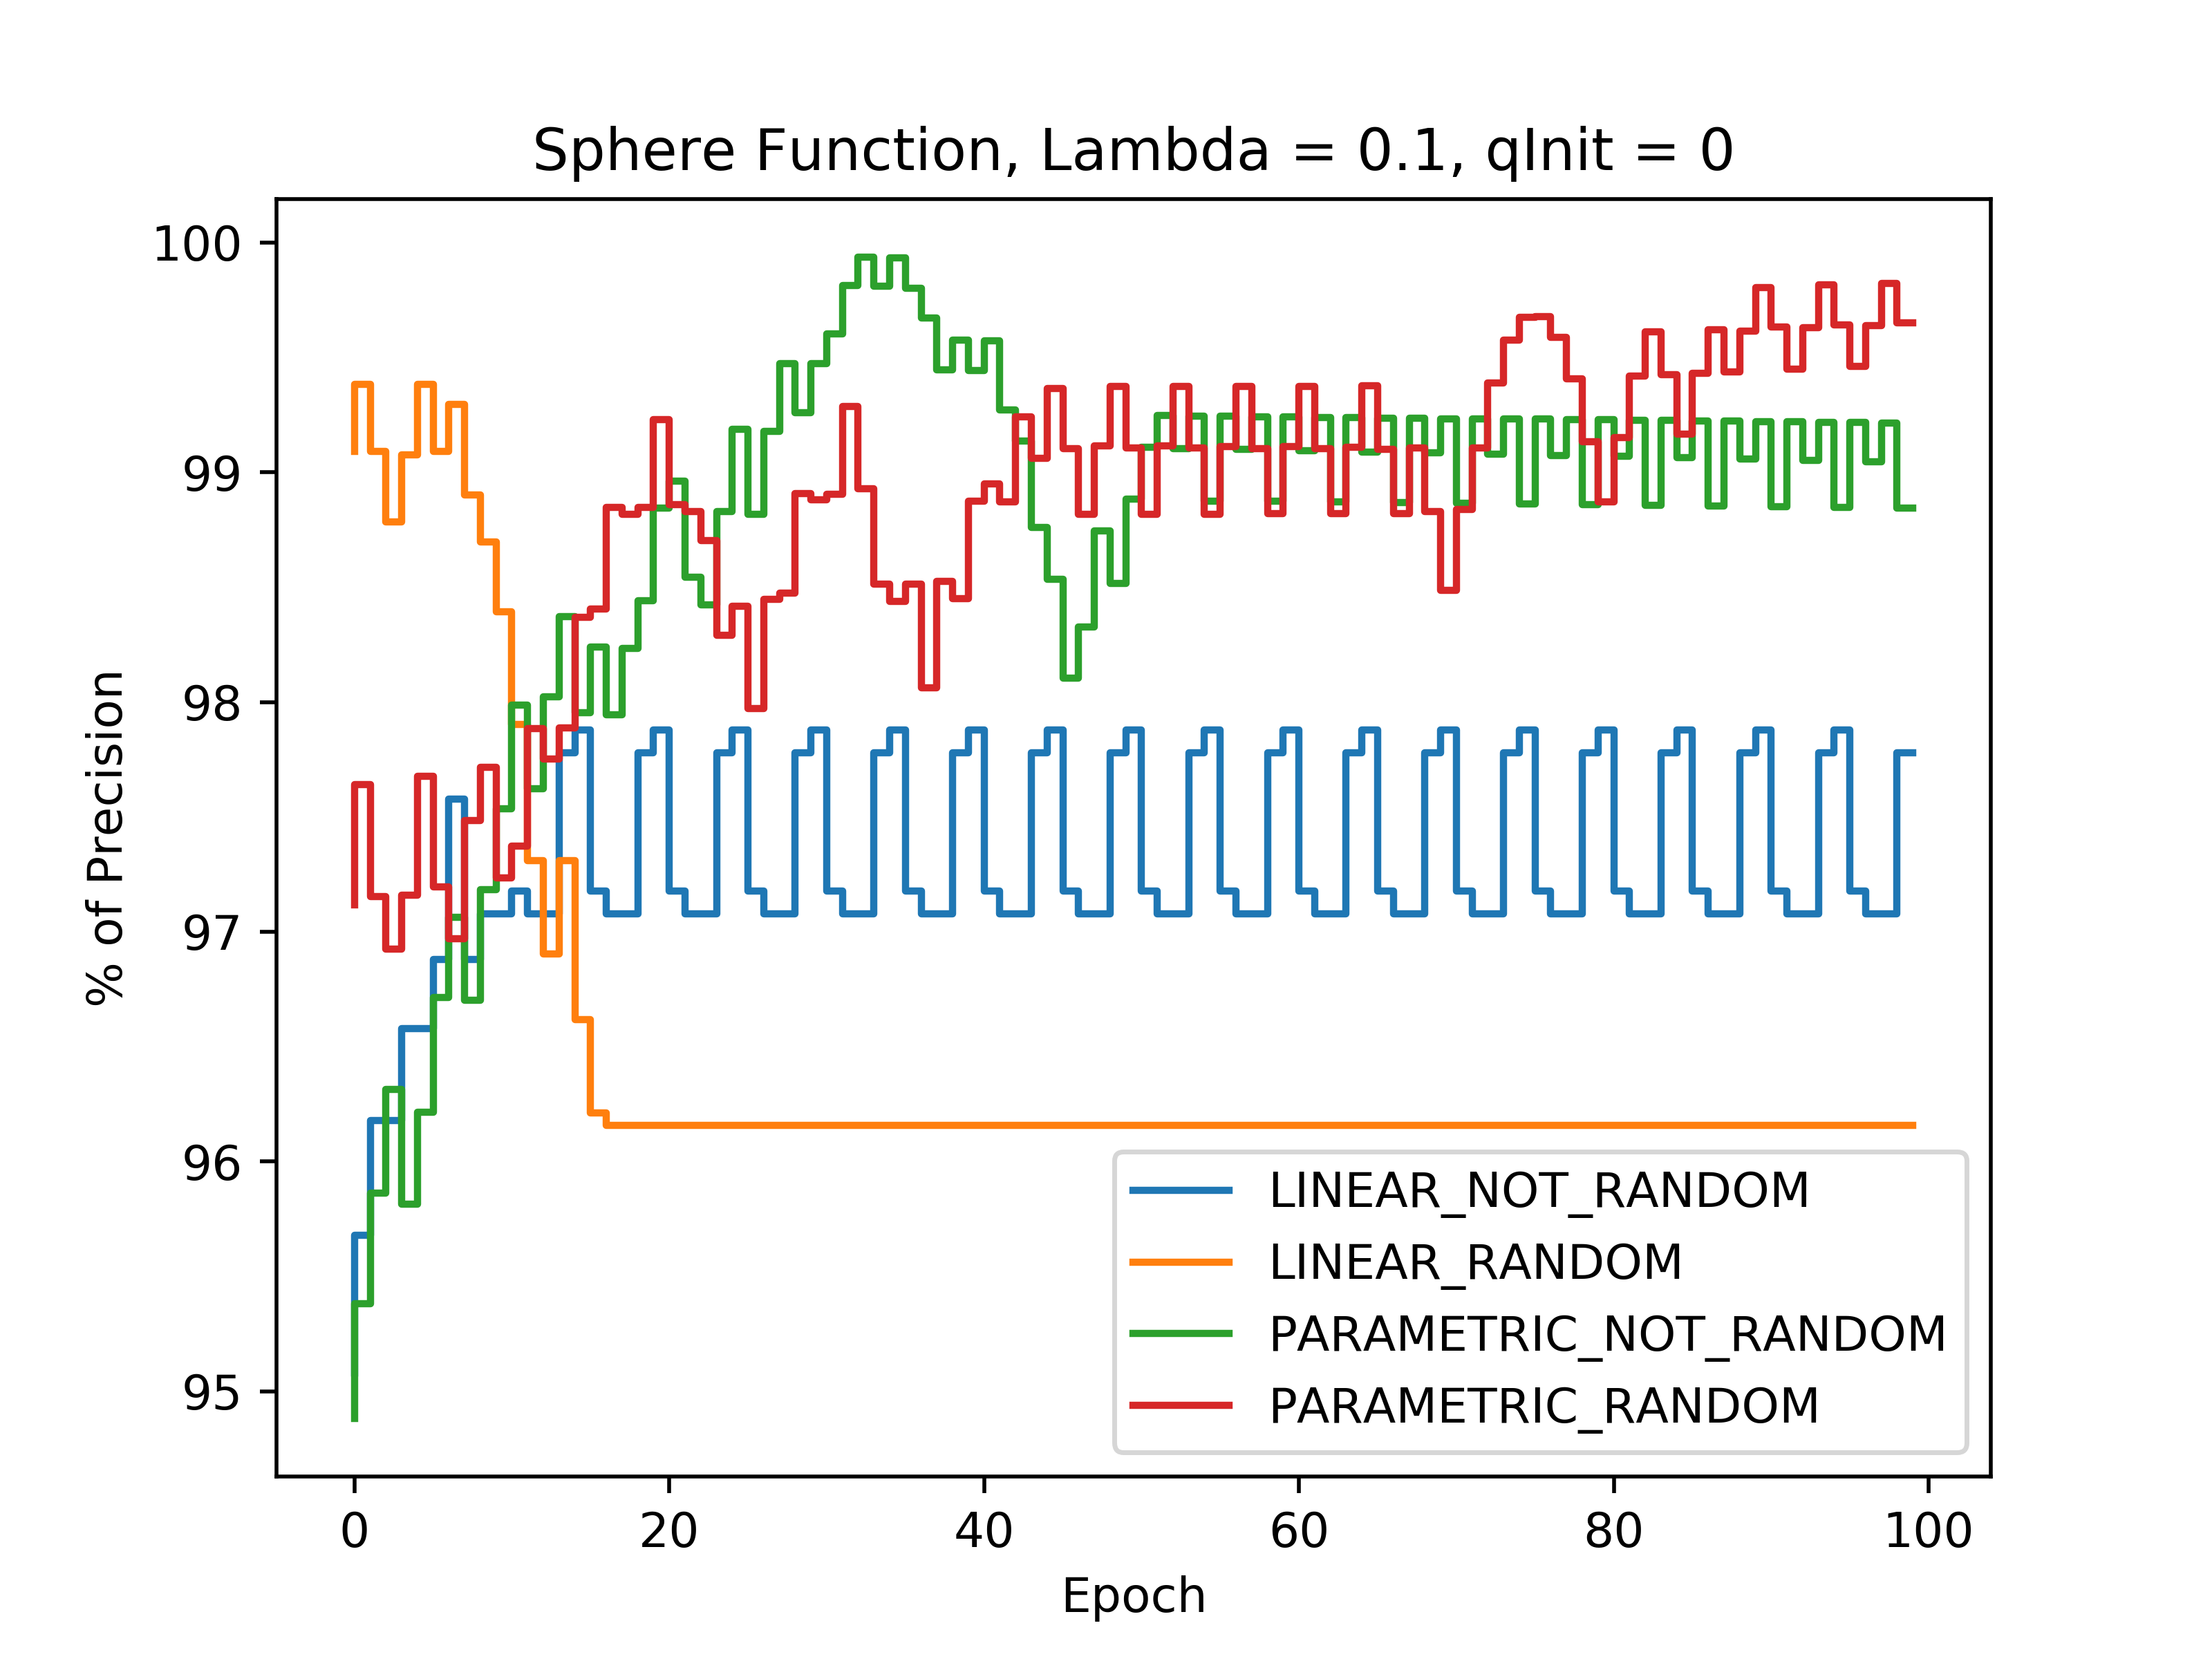
\includegraphics[width=0.4\textwidth]{SphereValueFunction}
		}\\
		\subfigure[]{%
			\label{fig:ParabolicGap}
			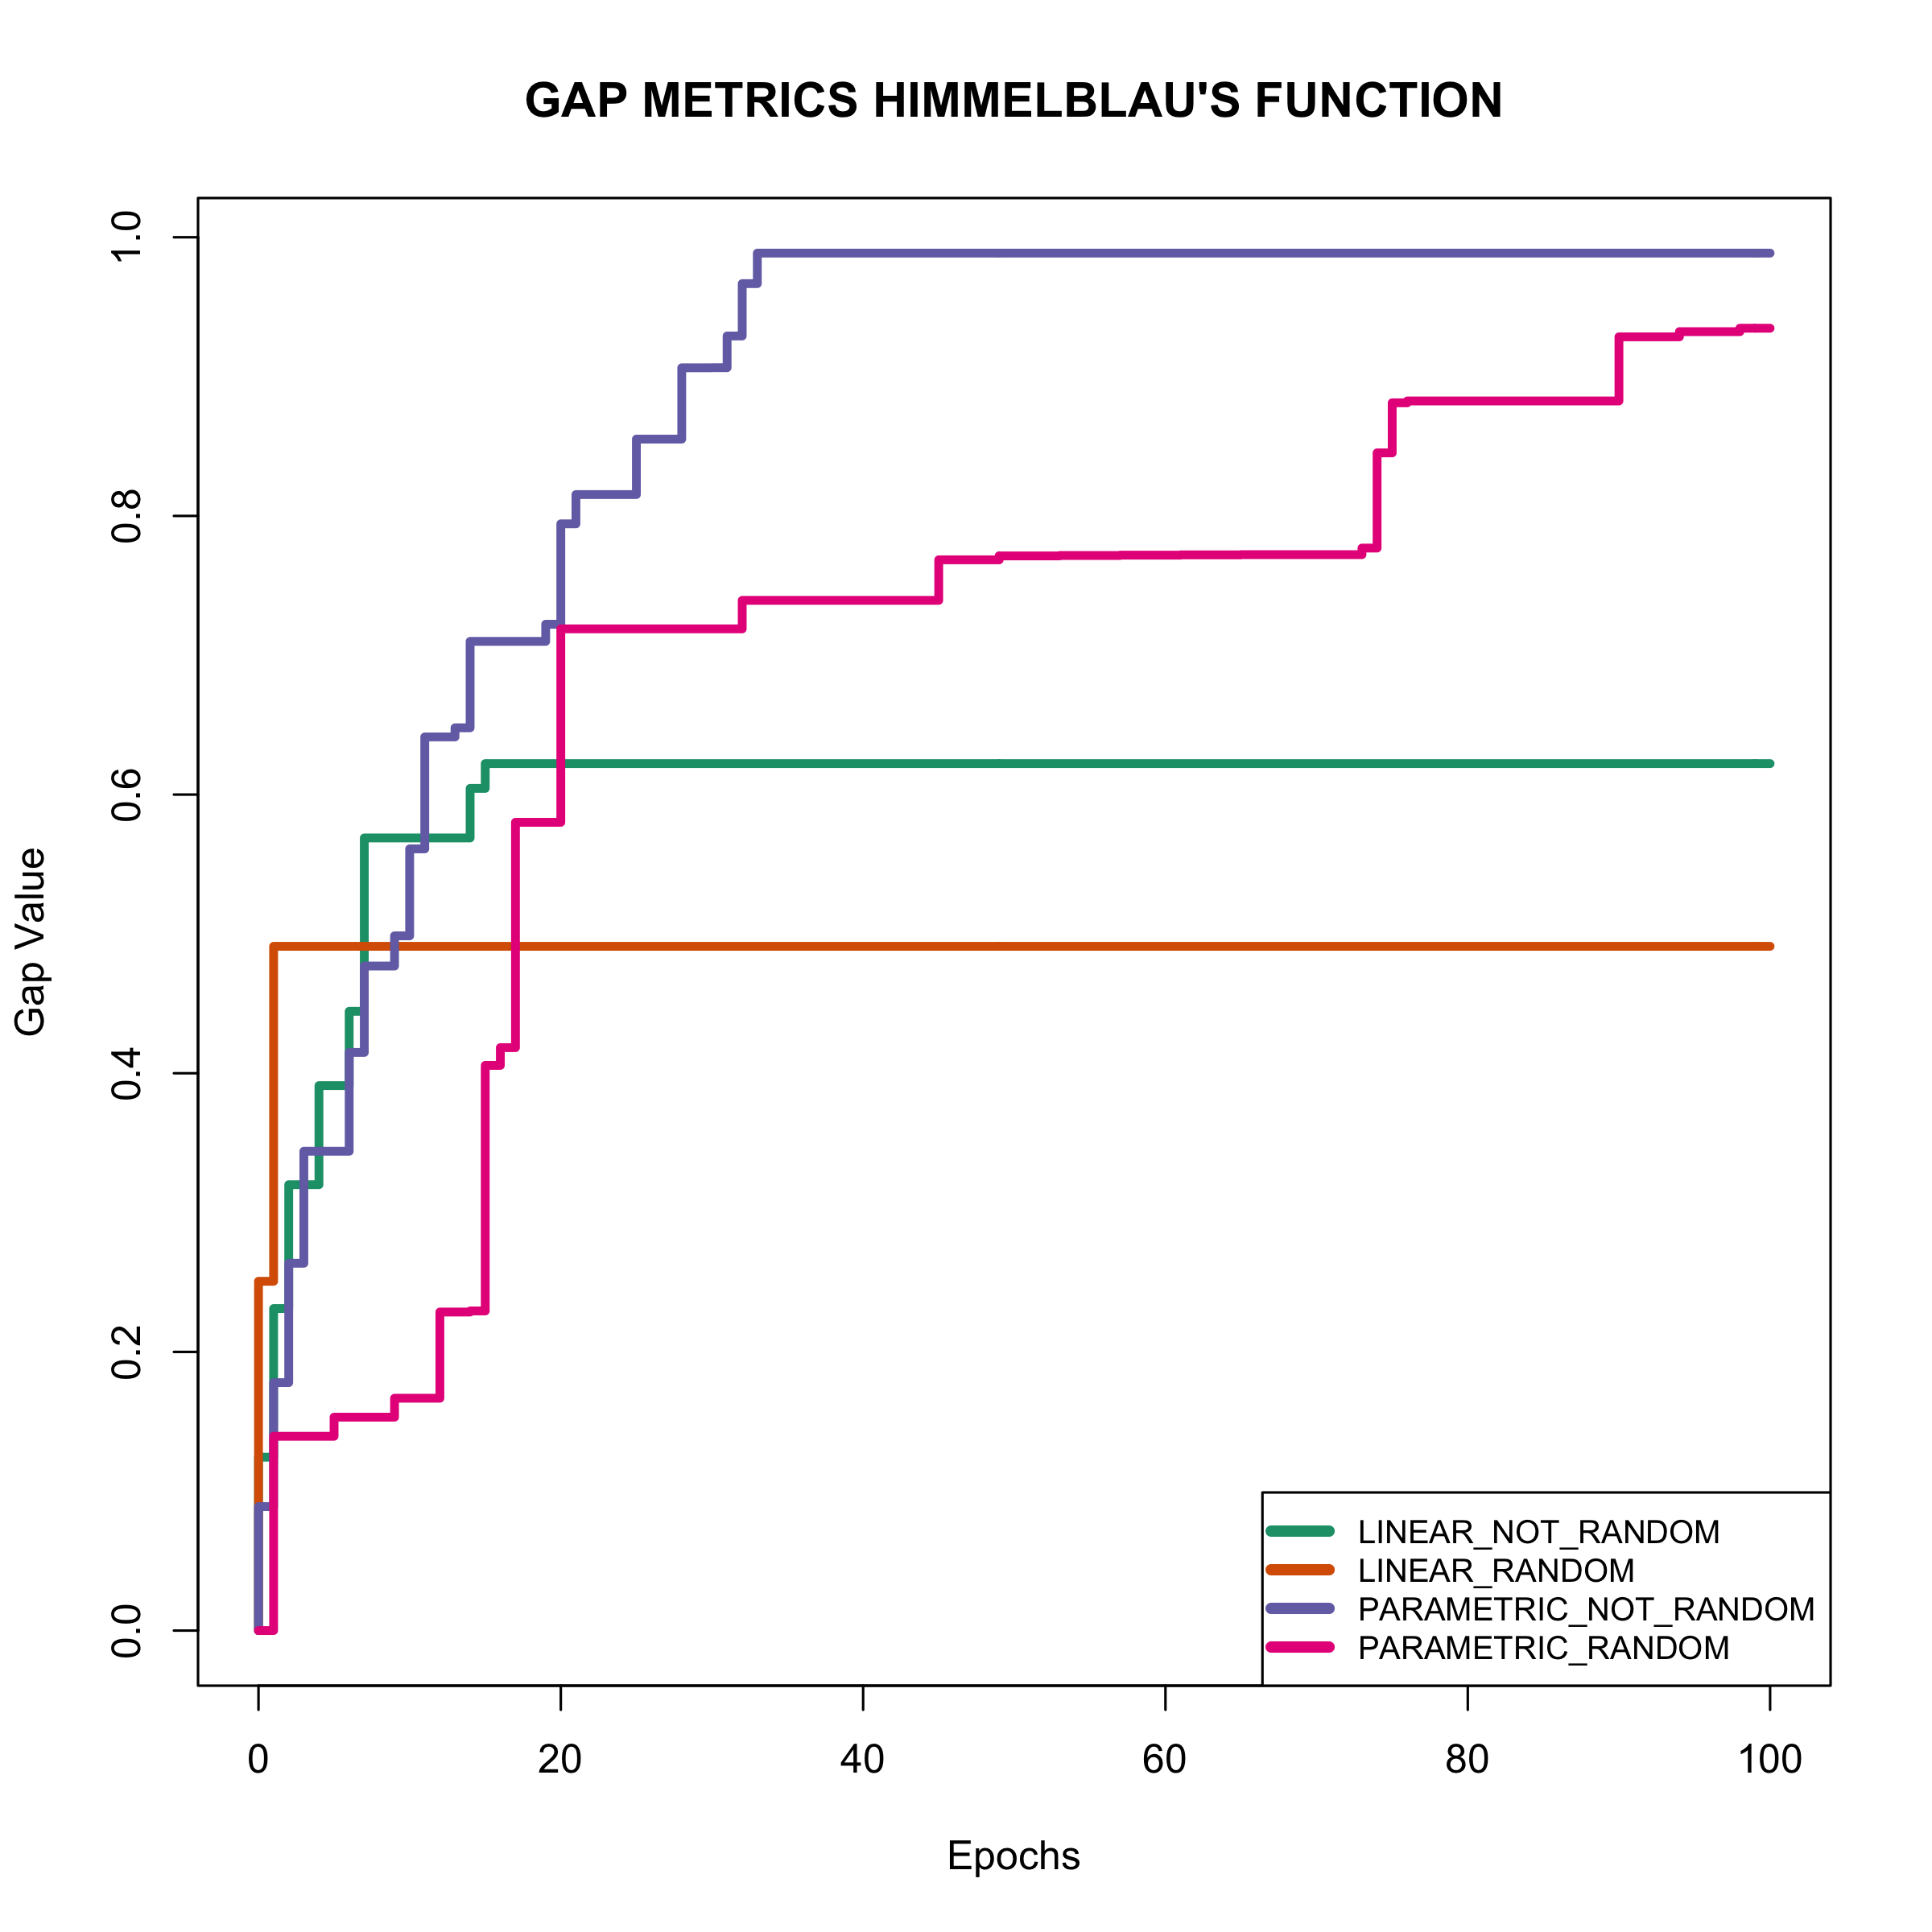
\includegraphics[width=0.4\textwidth]{ParabolicGap}
		} \\
		
	\end{center}
	\caption{
		Sphere Function.
	}
	\label{fig:ParabolicResults}
\end{figure}


\subsection{Sphere Function} Before starting to analyse performances of different declinations of {\tt SARSA($\lambda$)} algorithm in maximizing the Sphere function, it is important to underline that the starting point for the current function in non-random declinations is $(0, 0)$. The reason for this choice is that $f(300, 300)$ is itself the maximum of the function. \\

Plot (a) of figure ~\ref{fig:ParabolicResults} graphically represents performances of the four possible declinations of {\tt SARSA($\lambda$)} algorithm obtained considering the \textit{Euclidean distance metric}. Looking at the {\tt linear, not random} declination it is possible to note a constant, high Euclidean difference between the agent's position and the global maximum. This distance never decreases and still from the first epochs, a recurrent pattern starts to be developed. The inefficiency of the algorithm's declination depends on an inadequate training space. The relationship between different explored states and total possible states does not permit the agent to develop an efficient policy. Bad performance's results of the current declination are also certified by an high metric's average (table $5.3$). On the other hand the great stability of this declination is underlined by the lowest standard deviation of the set (table $5.3$).

{\tt Linear, random} declination starts from a point relatively close to the maximum, but, one more time, the inadequate training space prevents its to develop a rally optimal policy. This declination is the less efficient one with an average Euclidean distance from the maximum of $328.9$ pixels.

Better performances can be registered looking at parametric declinations of the algorithm. The {\tt parametric, not random} declination starts with a physiological high Euclidean difference from the maximum. It rapidly decreases until the thirty-fifth epoch and then it has another soft increase. Starting from the fifty-fifth epoch a recurrent pattern starts to be developed. Despite of the fact that this declination is the most unstable one with a standard deviation of $67.9$ (table $5.3$), it has one of the lowest average Euclidean distance from the maximum. 

The {\tt parametric, random} declination of {\tt SARSA($\lambda$)} algorithm has the best performance of the set. After a starting, considerable instability it reaches an Euclidean difference of around fifty pixels. The good performance is also proved by the fact that the average Euclidean distance from the maximum is $185.3$ pixels. \\

\begin{table}[h!]
	\centering
	\resizebox{\linewidth}{!} {
	\begin{tabular}{c| cccccc} 
		\hline \textbf{Sphere Function}
		& \textbf{Mean (pixels)} & \textbf{Standard deviation} \\ 
		\hline Linear not Random
		& $293.2$ &\cellcolor{red!25} $25.6$  \\ 
		\hline Linear Random
		& $328.9$ & $56.3$ \\ 
		\hline Parametric not Random
		& $190.7$ & $67.9$ \\ 
		\hline Parametric Random
		& \cellcolor{red!25} $185.3$ & $58.0$ \\ 
		\hline 
	\end{tabular} 
}
\label{ParabolicTabEuclidean}
\caption{Euclidean Metric's Performances}
\end{table}

Plot (b) of figure ~\ref{fig:ParabolicResults} graphically represents performances of the four possible declinations of {\tt SARSA($\lambda$)} algorithm obtained considering the \textit{Function Proximity in Percentage} metric. 

The {\tt linear, not random} declination starts from a value function's proximity of about $97.5\%$ from the maximum. It is completely unable to improve this percentage. Already starting from the first epochs it develops a recurrent pattern. This behaviour allows its to have the lowest standard deviation of the declinations' set (table $5.4$). Unfortunately the value function's proximity mean is the second lowest one. 
 
The {\tt linear, random} declination starts from a very high value function's proximity level. Because of an inadequate training space it decreases until the twentieth epoch. Starting from this epoch it stars to stabilize. Effects of this behaviour on the average value function's proximity to the maximum and on average standard deviation are relevant.
 
The {\tt parametric, not random} declination is the most unstable one. It starts with a low value function's proximity level and slowly grows achieving peaks of about $100\%$. Starting from the fiftieth epoch it stabilizes developing a recurrent pattern. The initial high instability has effects on average value function's proximity variance making its the highest one (table $5.4$).
 
The {\tt parametric, random} declination of {\tt SARSA($\lambda$)} algorithm is the most efficient one. It starts with a value function's proximity level of about $97\%$ and slowly grows first stabilizing around $99\%$ and than growing more achieving peaks of $99.8\%$. Looking at table $5.4$ it is possible to note that the average value function's proximity is the highest one with a level of $98.8\%$.
 
In this case it is possible to underline that parametric declinations do better than linear ones. In particular the random starting position allows the agent to develop a better policy. The main reason of the failure of non random declinations is the reduced training space compared to the distance between the starting point and the maximum.

\begin{table}[h!]
	\centering
	\resizebox{\linewidth}{!} {
	\begin{tabular}{c| cccccc} 
		\hline \textbf{Sphere Function}
		& \textbf{Mean (\%)} & \textbf{Standard deviation} \\ 
		\hline Linear not Random
		& $97.3$ & \cellcolor{green!25}$0.49$ \\ 
		\hline Linear Random
		& $95.5$ & $0.92$ \\ 
		\hline Parametric not Random
		& $98.7$ & $0.98$ \\ 
		\hline Parametric Random
		& \cellcolor{green!25}$98.8$ & $0.72$ \\ 
		\hline 
	\end{tabular} 
}
\label{ParabolicTabProximity}
\caption{Function Proximity in Percentage.} 
\end{table}

Plot (c) of figure ~\ref{fig:ParabolicResults} graphically represents performances of the four possible declinations of {\tt SARSA($\lambda$)} algorithm obtained using the \textit{Gap metric}. According to this plot the most effective declination of {\tt SARSA($\lambda$)} algorithm in finding the maximum is the {\tt parametric, not random} one. Looking at table $5.9$ it is possible to note that {\tt parametric, not random} declination achieves point $(-1.033, -1.099)$ with a value function of $3557.722$ out of $3560.0$.

\begin{figure}[h!]
	\begin{center}
		\subfigure[]{%
			\label{fig:BealeDifference}
			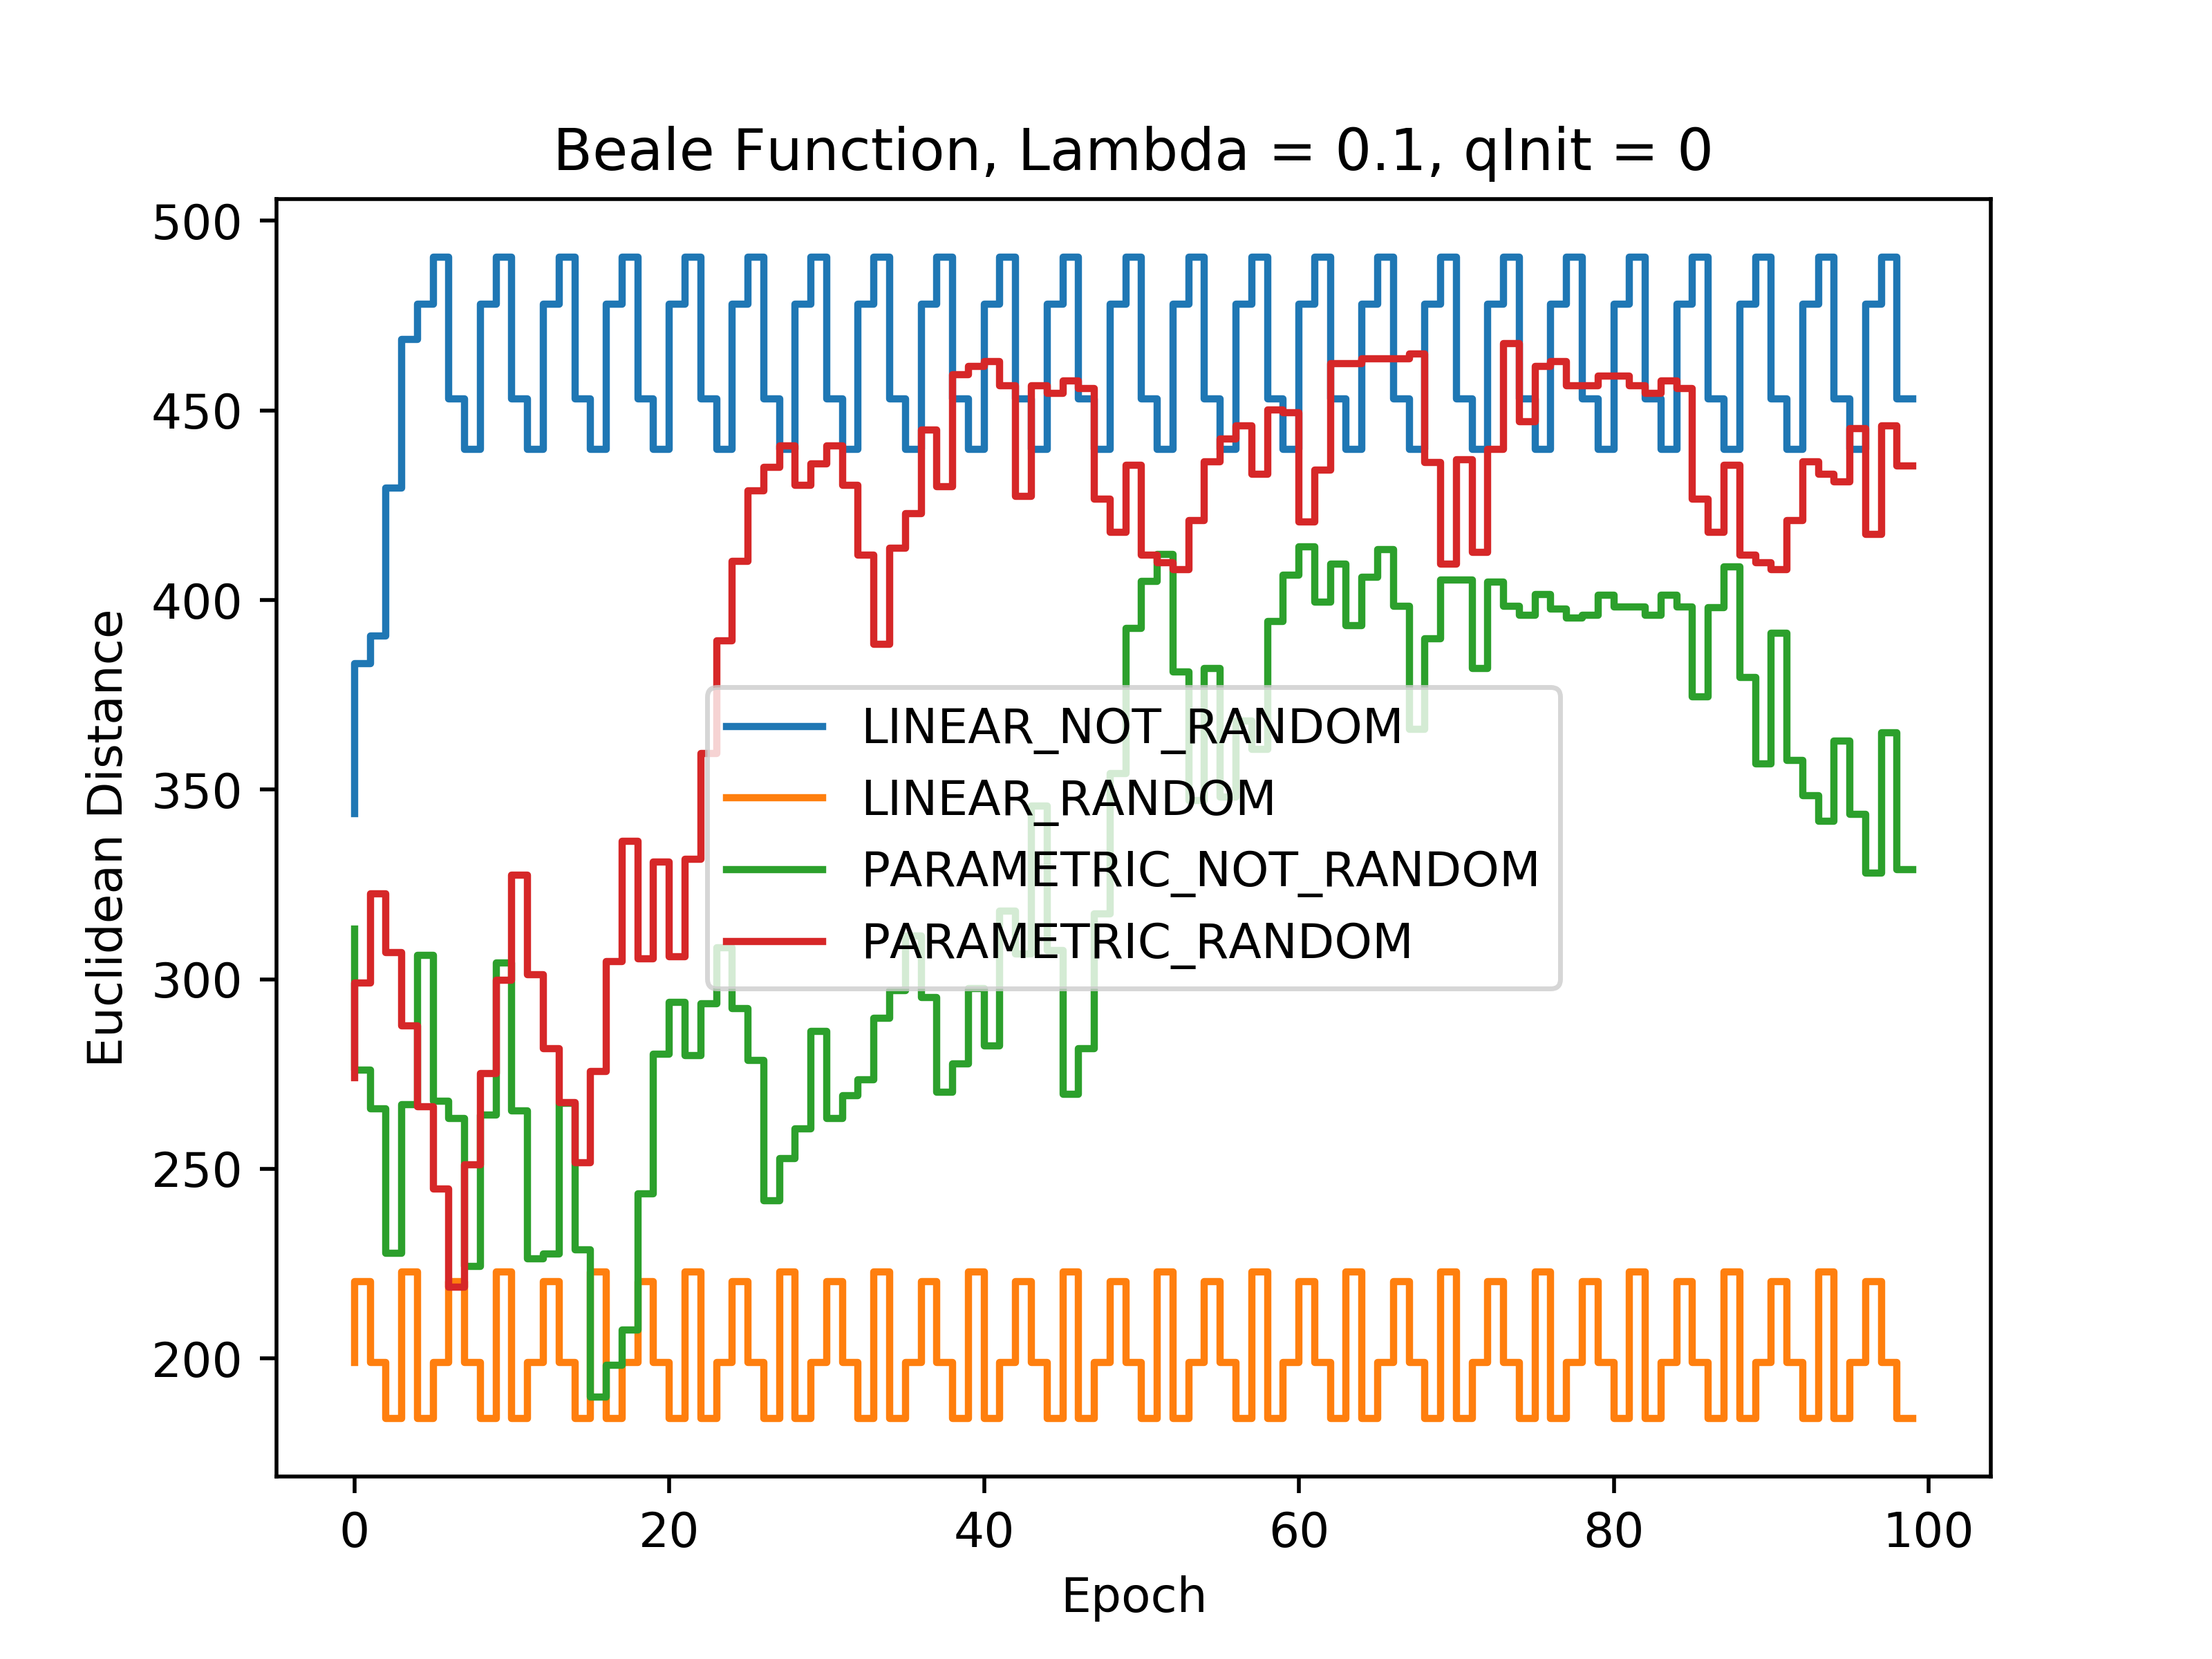
\includegraphics[width=0.4\textwidth]{BealeDifference}
		}
		\subfigure[]{%
			\label{fig:BealeValueFunction}
			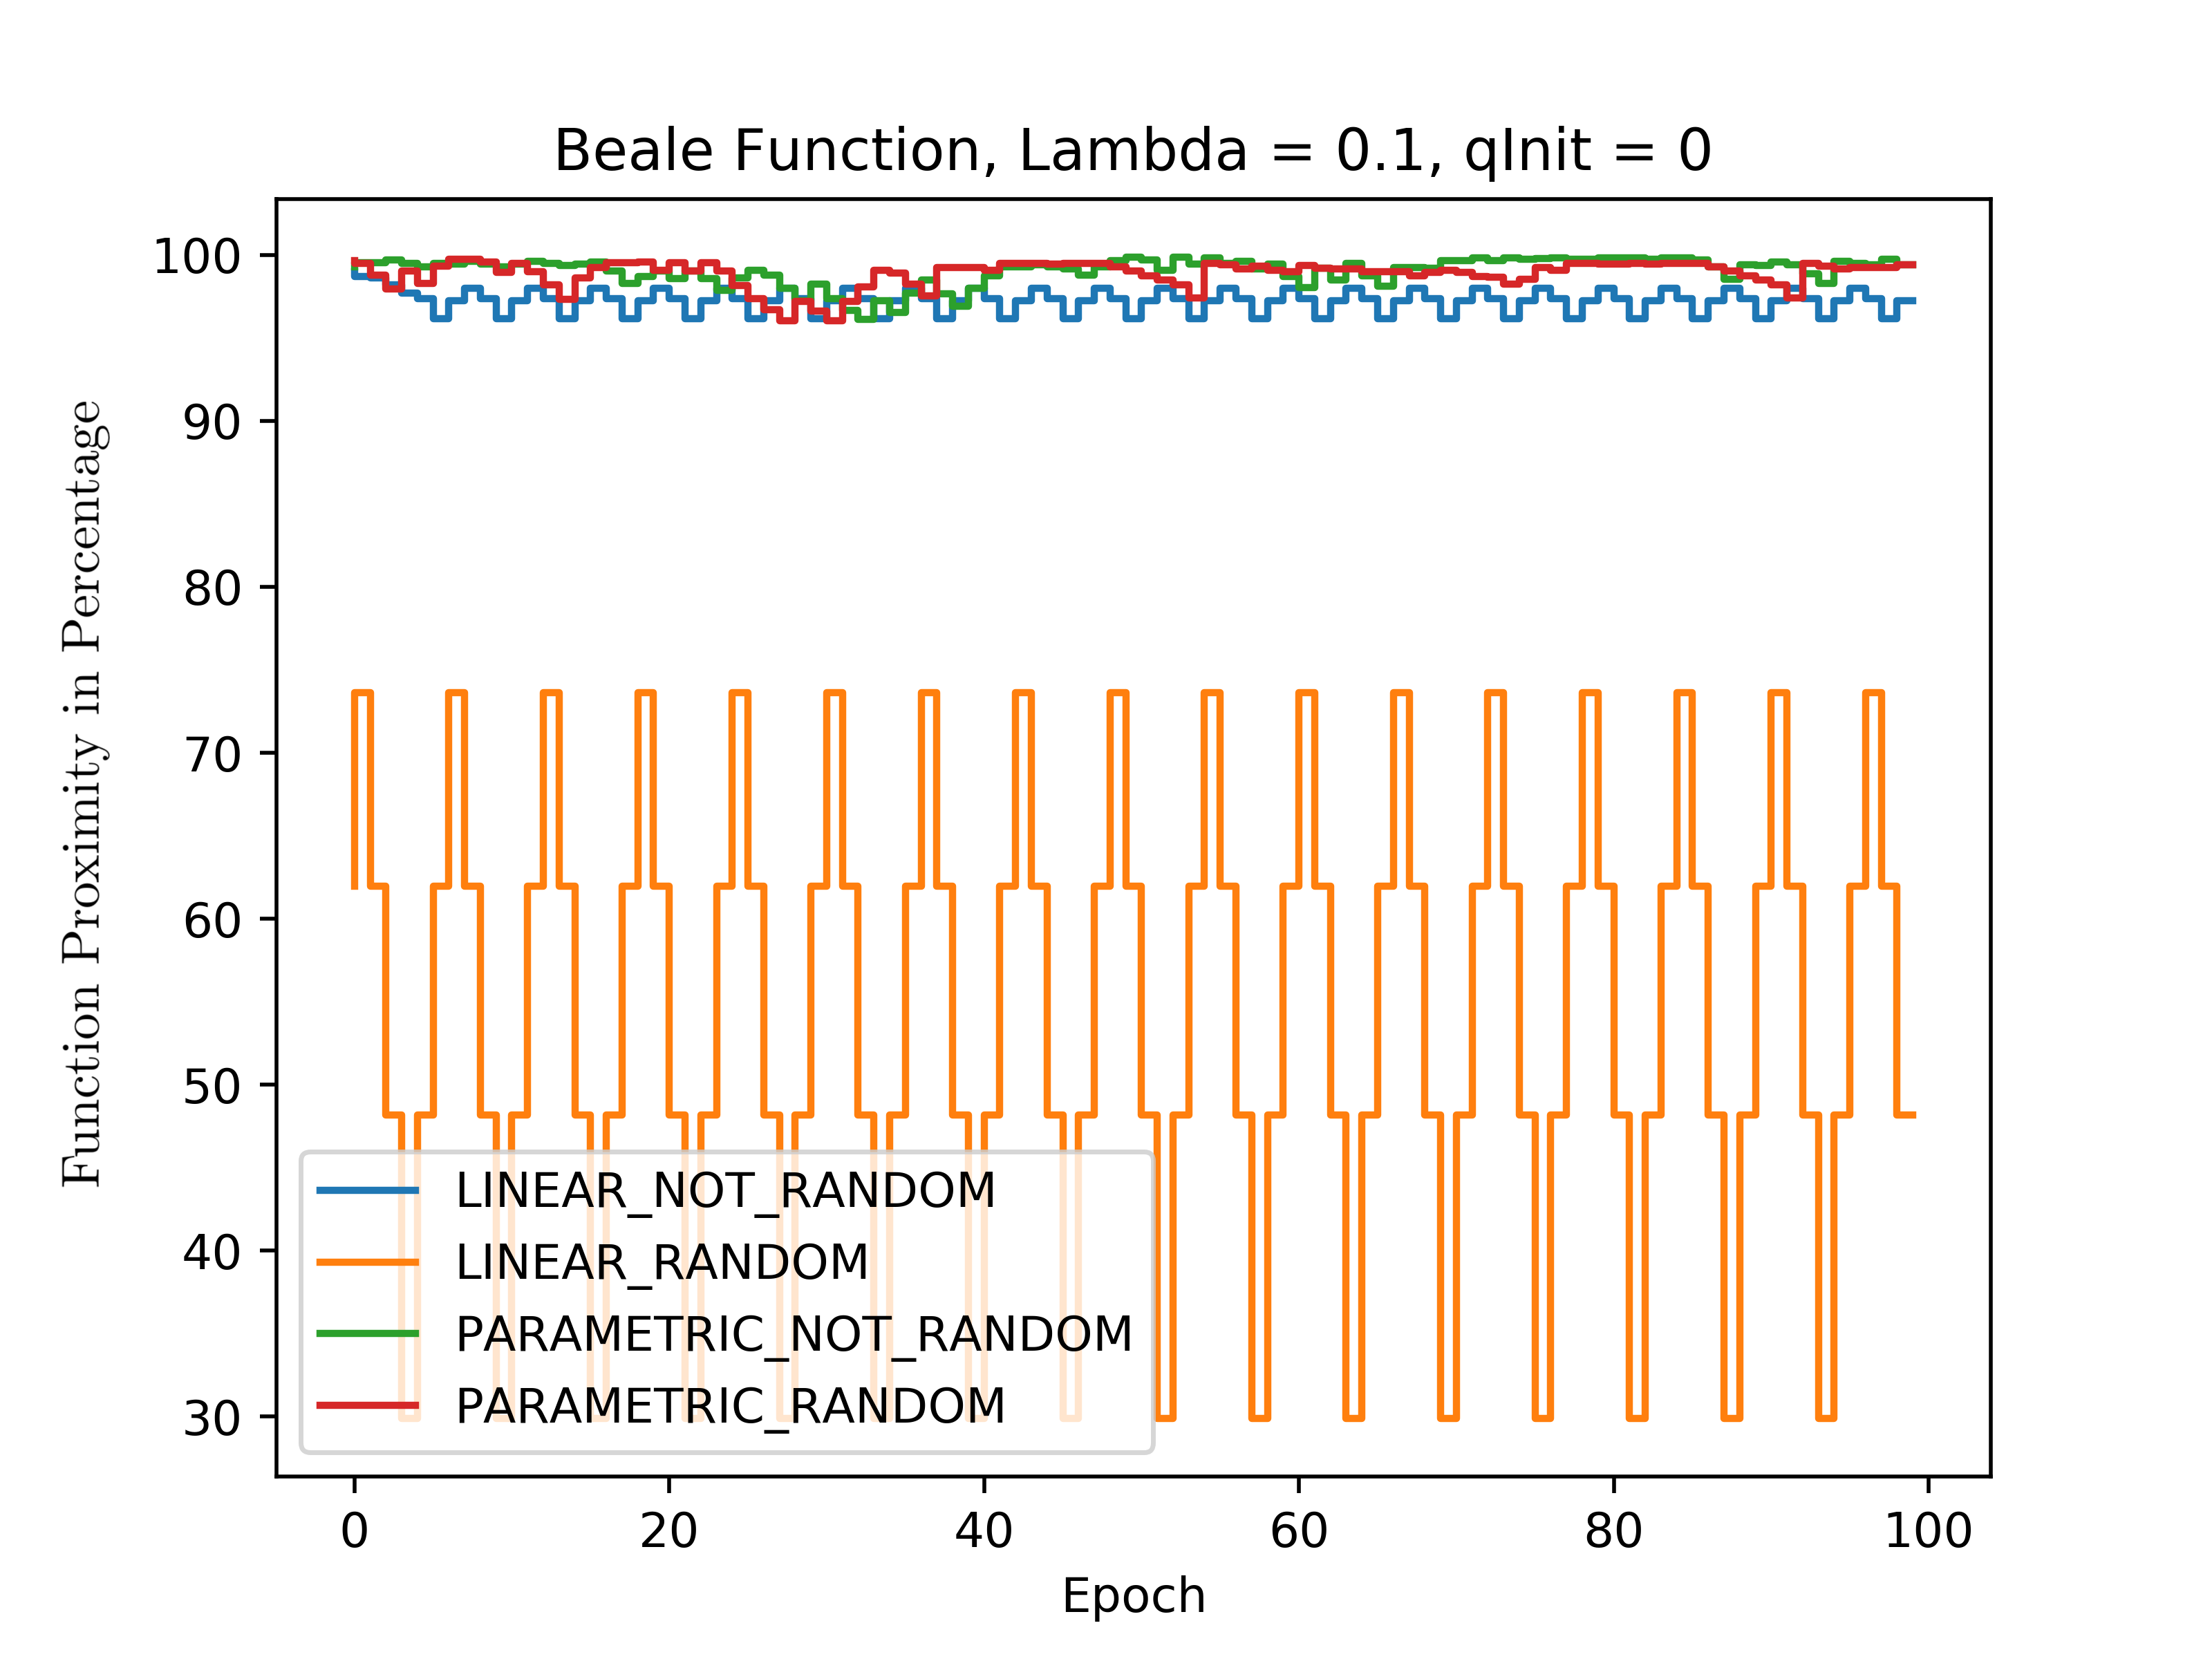
\includegraphics[width=0.4\textwidth]{BealeValueFunction}
		}\\
		\subfigure[]{%
			\label{fig:BealeGap}
			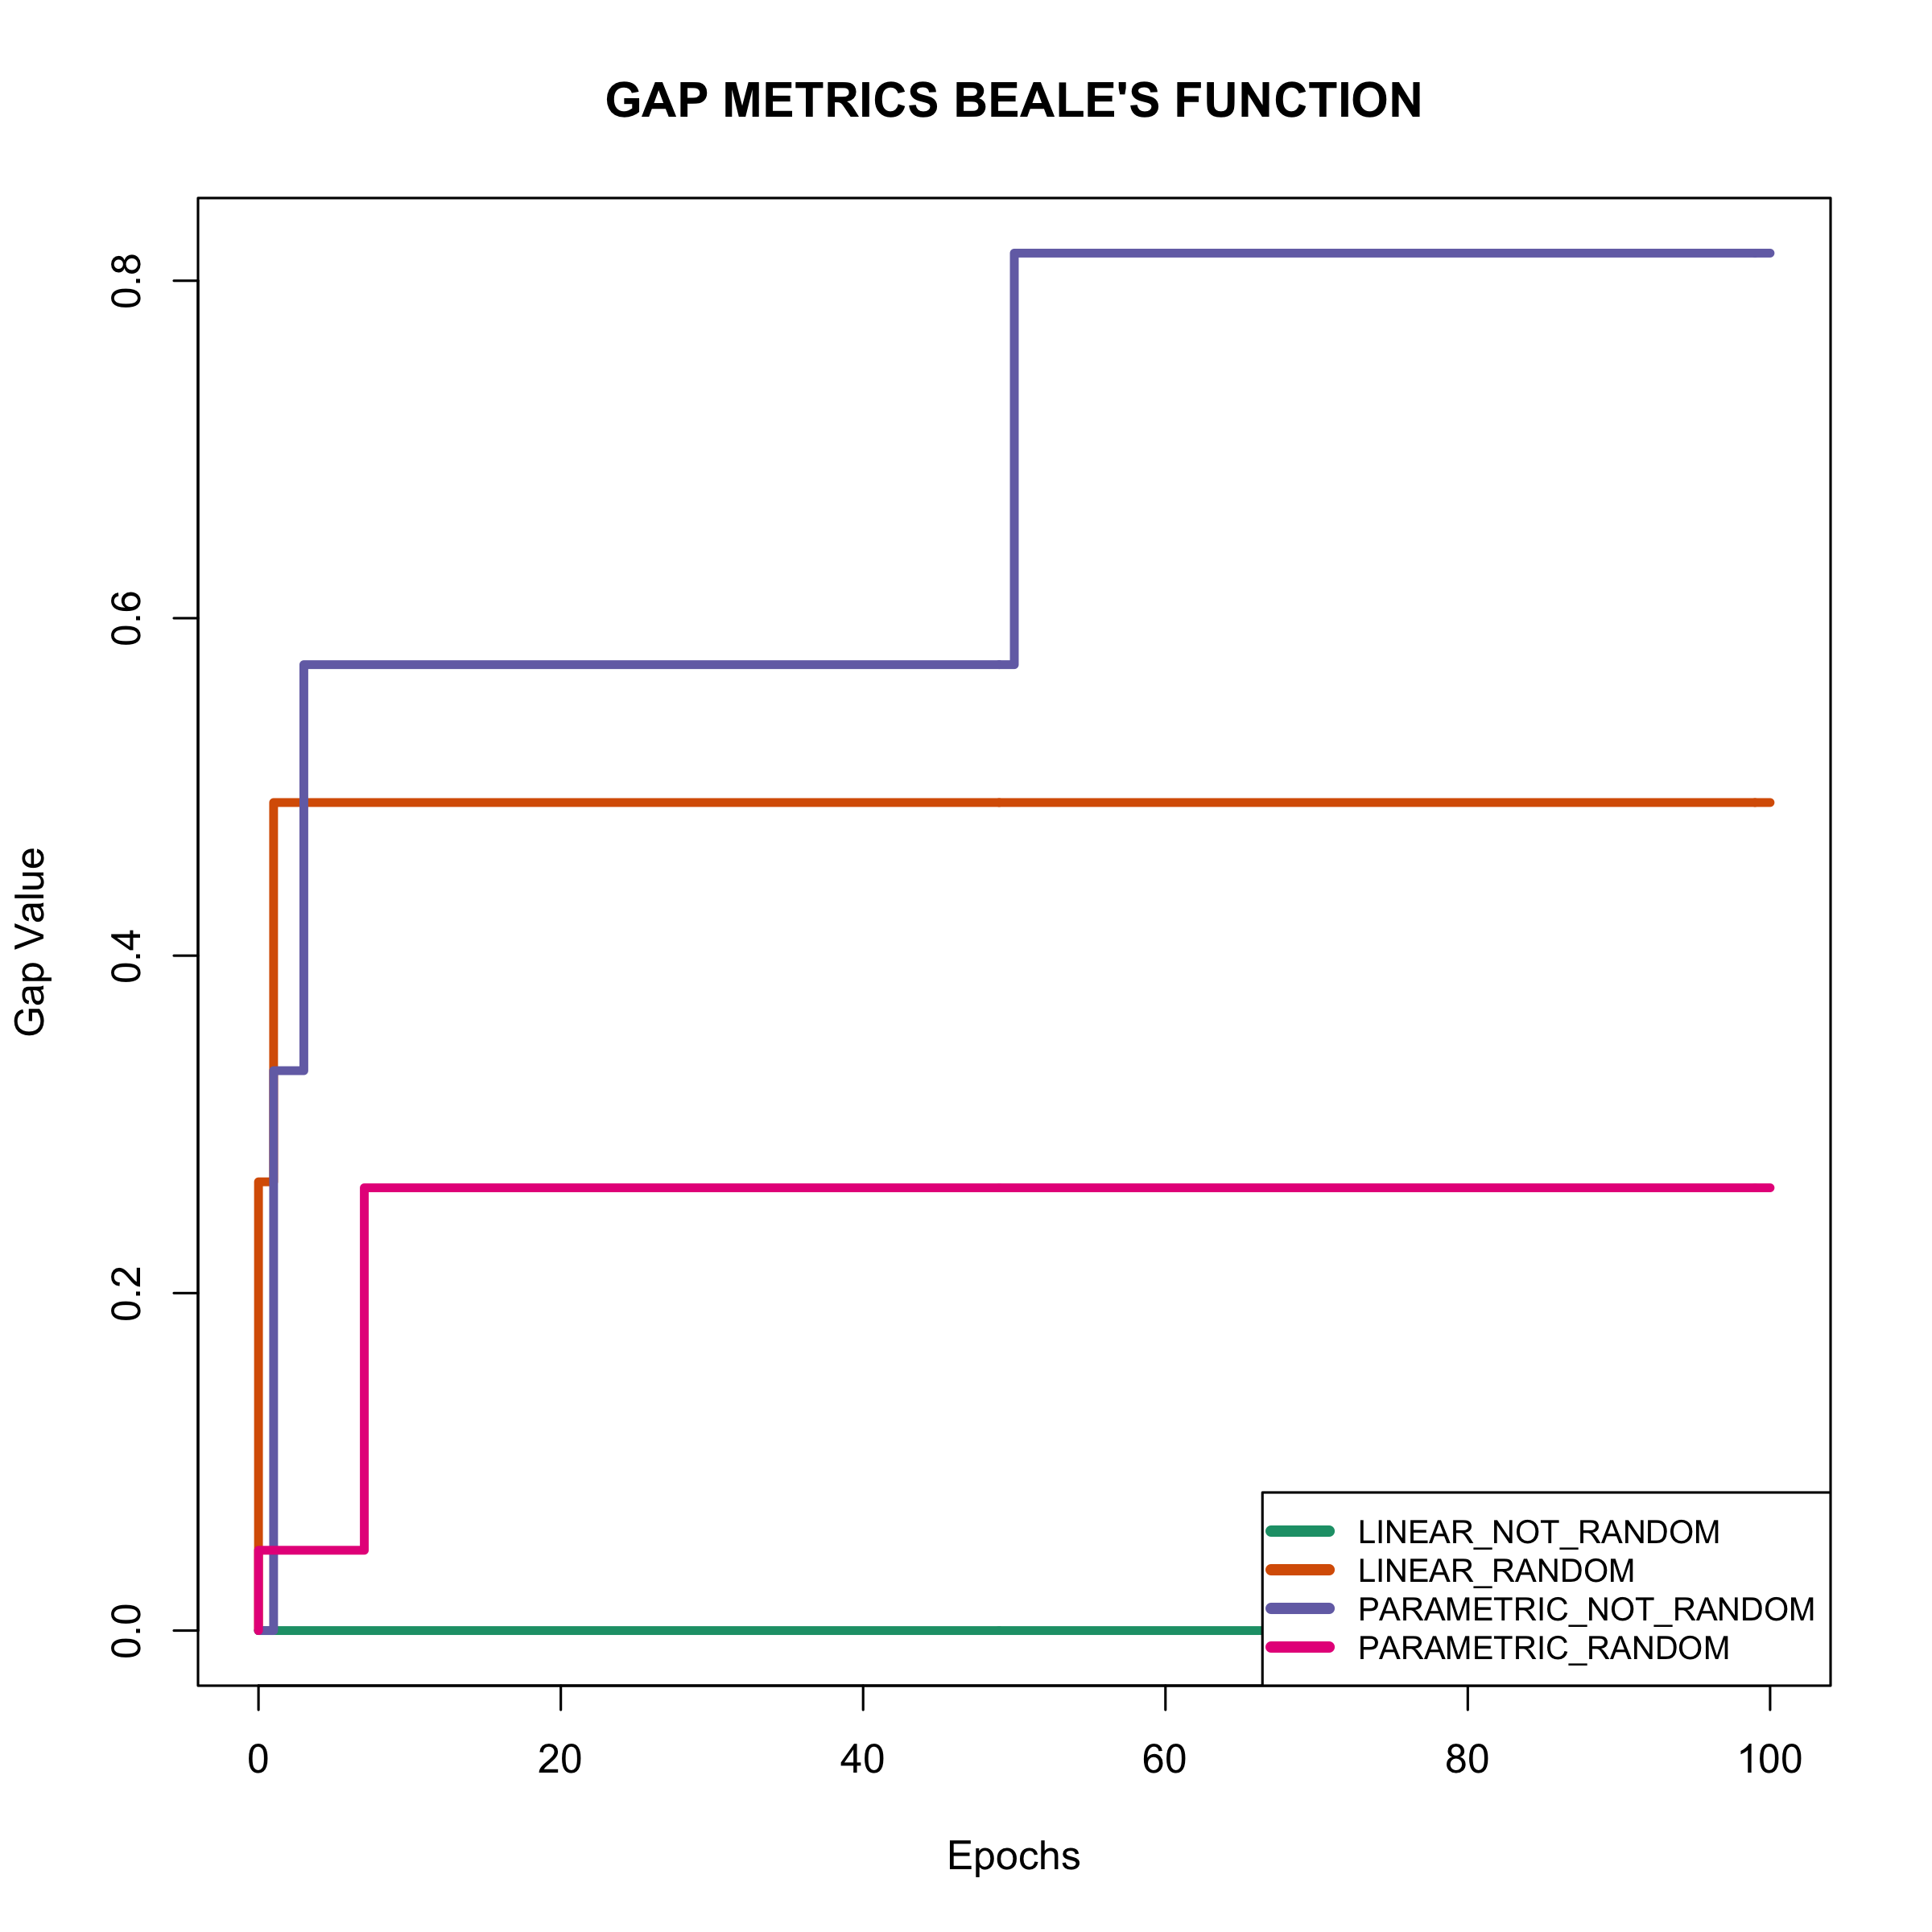
\includegraphics[width=0.4\textwidth]{BealeGap}
		} \\
		
	\end{center}
	\caption{
		Beale Function.
	}
	\label{fig:BealeResults}
\end{figure}

\subsection{Beale Function} Giving an overview to figure \ref{fig:BealeResults} it is possible to see that Beale Function represents the case in which {\tt SARSA($\lambda$)} algorithm' s declinations do worst. 

Plot (a) of figure \ref{fig:BealeResults} graphically represents performances of the four possible declinations of {\tt SARSA($\lambda$)} algorithm obtained considering the \textit{Euclidean distance metric}. Looking at the {\tt linear, not random} declination it is possible to note a growing performance' s worsening until tenth epoch. Starting from epoch ten algorithm's declination starts to stabilize developing a recurrent pattern. Using this declination, the average Euclidean distance from the maximum is $462.4$ pixels.

{\tt Linear, random} declination seems to be the one which performs better. Its average Euclidean distance from the maximum is $201.6$ pixels and its standard deviation is the lowest of the set with a value of $15.4$. This means that it has a relatively good stability. Looking at plot (a) what just said can be easily proved. The current declination starts from a point relatively near to the maximum and never departs from its developing a recurrent pattern.

Looking at {\tt parametric, not random} declination of  {\tt SARSA($\lambda$)} algorithm it is possible to note an high instability. In the very first epochs the distance between the starting point and the maximum slowly decreases, but starting from epoch thirty it starts to messily increase achieving a level near to $350$ pixels. This high instability is reflected also in the high level of standard deviation (table $5.5$).

{\tt Parametric, random} declination combines instability and inaccuracy. It starts from a distance of about $300$ pixels and messily increase its. Its performance is the worst one with an average Euclidean distance of $402.99$ pixels and a standard deviation of $66.6$ (table $5.5$).

Generally speaking it is possible to affirm that those bad performances are the result of an inadequate training space and of a particularly flat function's shape. In addition to this, as already explained, parametric declinations do worst than corresponding ones because of the reduced amount of movement at each epoch. The relatively better performance of {\tt linear, random} declination depends on the possibility to select a starting point closer to the maximum. \\

\begin{table}[h!]
\centering
\resizebox{\linewidth}{!} {
	\begin{tabular}{c| cccccc} 
		\hline \textbf{Beale Function}
		& \textbf{Mean (pixels)} & \textbf{Standard deviation} \\ 
		\hline Linear not Random
		& $462.4$ & $25.7$\\ 
		\hline Linear Random
		& \cellcolor{red!25}$201.6$ & \cellcolor{red!25}$15.4$\\ 
		\hline Parametric not Random
		& $329.8$ & $62.7$\\ 
		\hline Parametric Random
		& $402.99$ & $66.6$ \\ 
		\hline 
	\end{tabular} 
}
\label{BealeTabEuclidean}
\caption{Euclidean Metric's Performances}
\end{table}

Looking at plot (b) of figure \ref{fig:BealeResults} it is possible to note an inconsistency with what said until now. Only {\tt linear, random} configuration makes an highly swinging performance varying between a percentage of value function' s proximity of about $75\%$ to a percentage of $30\%$. All other declinations make performances around $100\%$ of value function' s proximity. Even looking at table $5.6$ this impression is proved by the high standard deviation of {\tt linear, random} configuration and by the high average of value function' s proximity of all other declinations. These apparently good performances depends on the function' s shape that is very flat. 

\begin{table}[h!]
	\centering
	\resizebox{\linewidth}{!} {
		\begin{tabular}{c| cccccc} 
			\hline \textbf{Beale Function}
			& \textbf{Mean (\%)} & \textbf{Standard deviation} \\ 
			\hline Linear not Random
			& $97.25$ & \cellcolor{green!25}$0.70$\\ 
			\hline Linear Random
			& $54.26$ & $13.89$\\ 
			\hline Parametric not Random
			& \cellcolor{green!25}$99.06$ & $0.81$ \\ 
			\hline Parametric Random
			& $98.88$ & $0.798$ \\ 
			\hline 
		\end{tabular} 
}
	\caption{Function Proximity in Percentage.} 
	\label{BealeTabProximity}
\end{table}

Deception can also be revealed by observing plot (c) of figure \ref{fig:BealeResults}. The relatively best performing declination is the {\tt parametric, not random} one which achieves an effectiveness in finding the maximum of about $0.8$ out of $1.0$. It is also proved by table $5.9$. {\tt Parametric, not random} declination achieves point $(-0.77, 1.5599)$ with a value function of $1997.392$ out of $2000$. The worst performing one is the {\tt linear, not random} declination with a constant \textit{Gap value} equals to $0$.

\begin{figure}[h!]
	\begin{center}
		\subfigure[]{%
			\label{fig:StyblinskiDifference}
			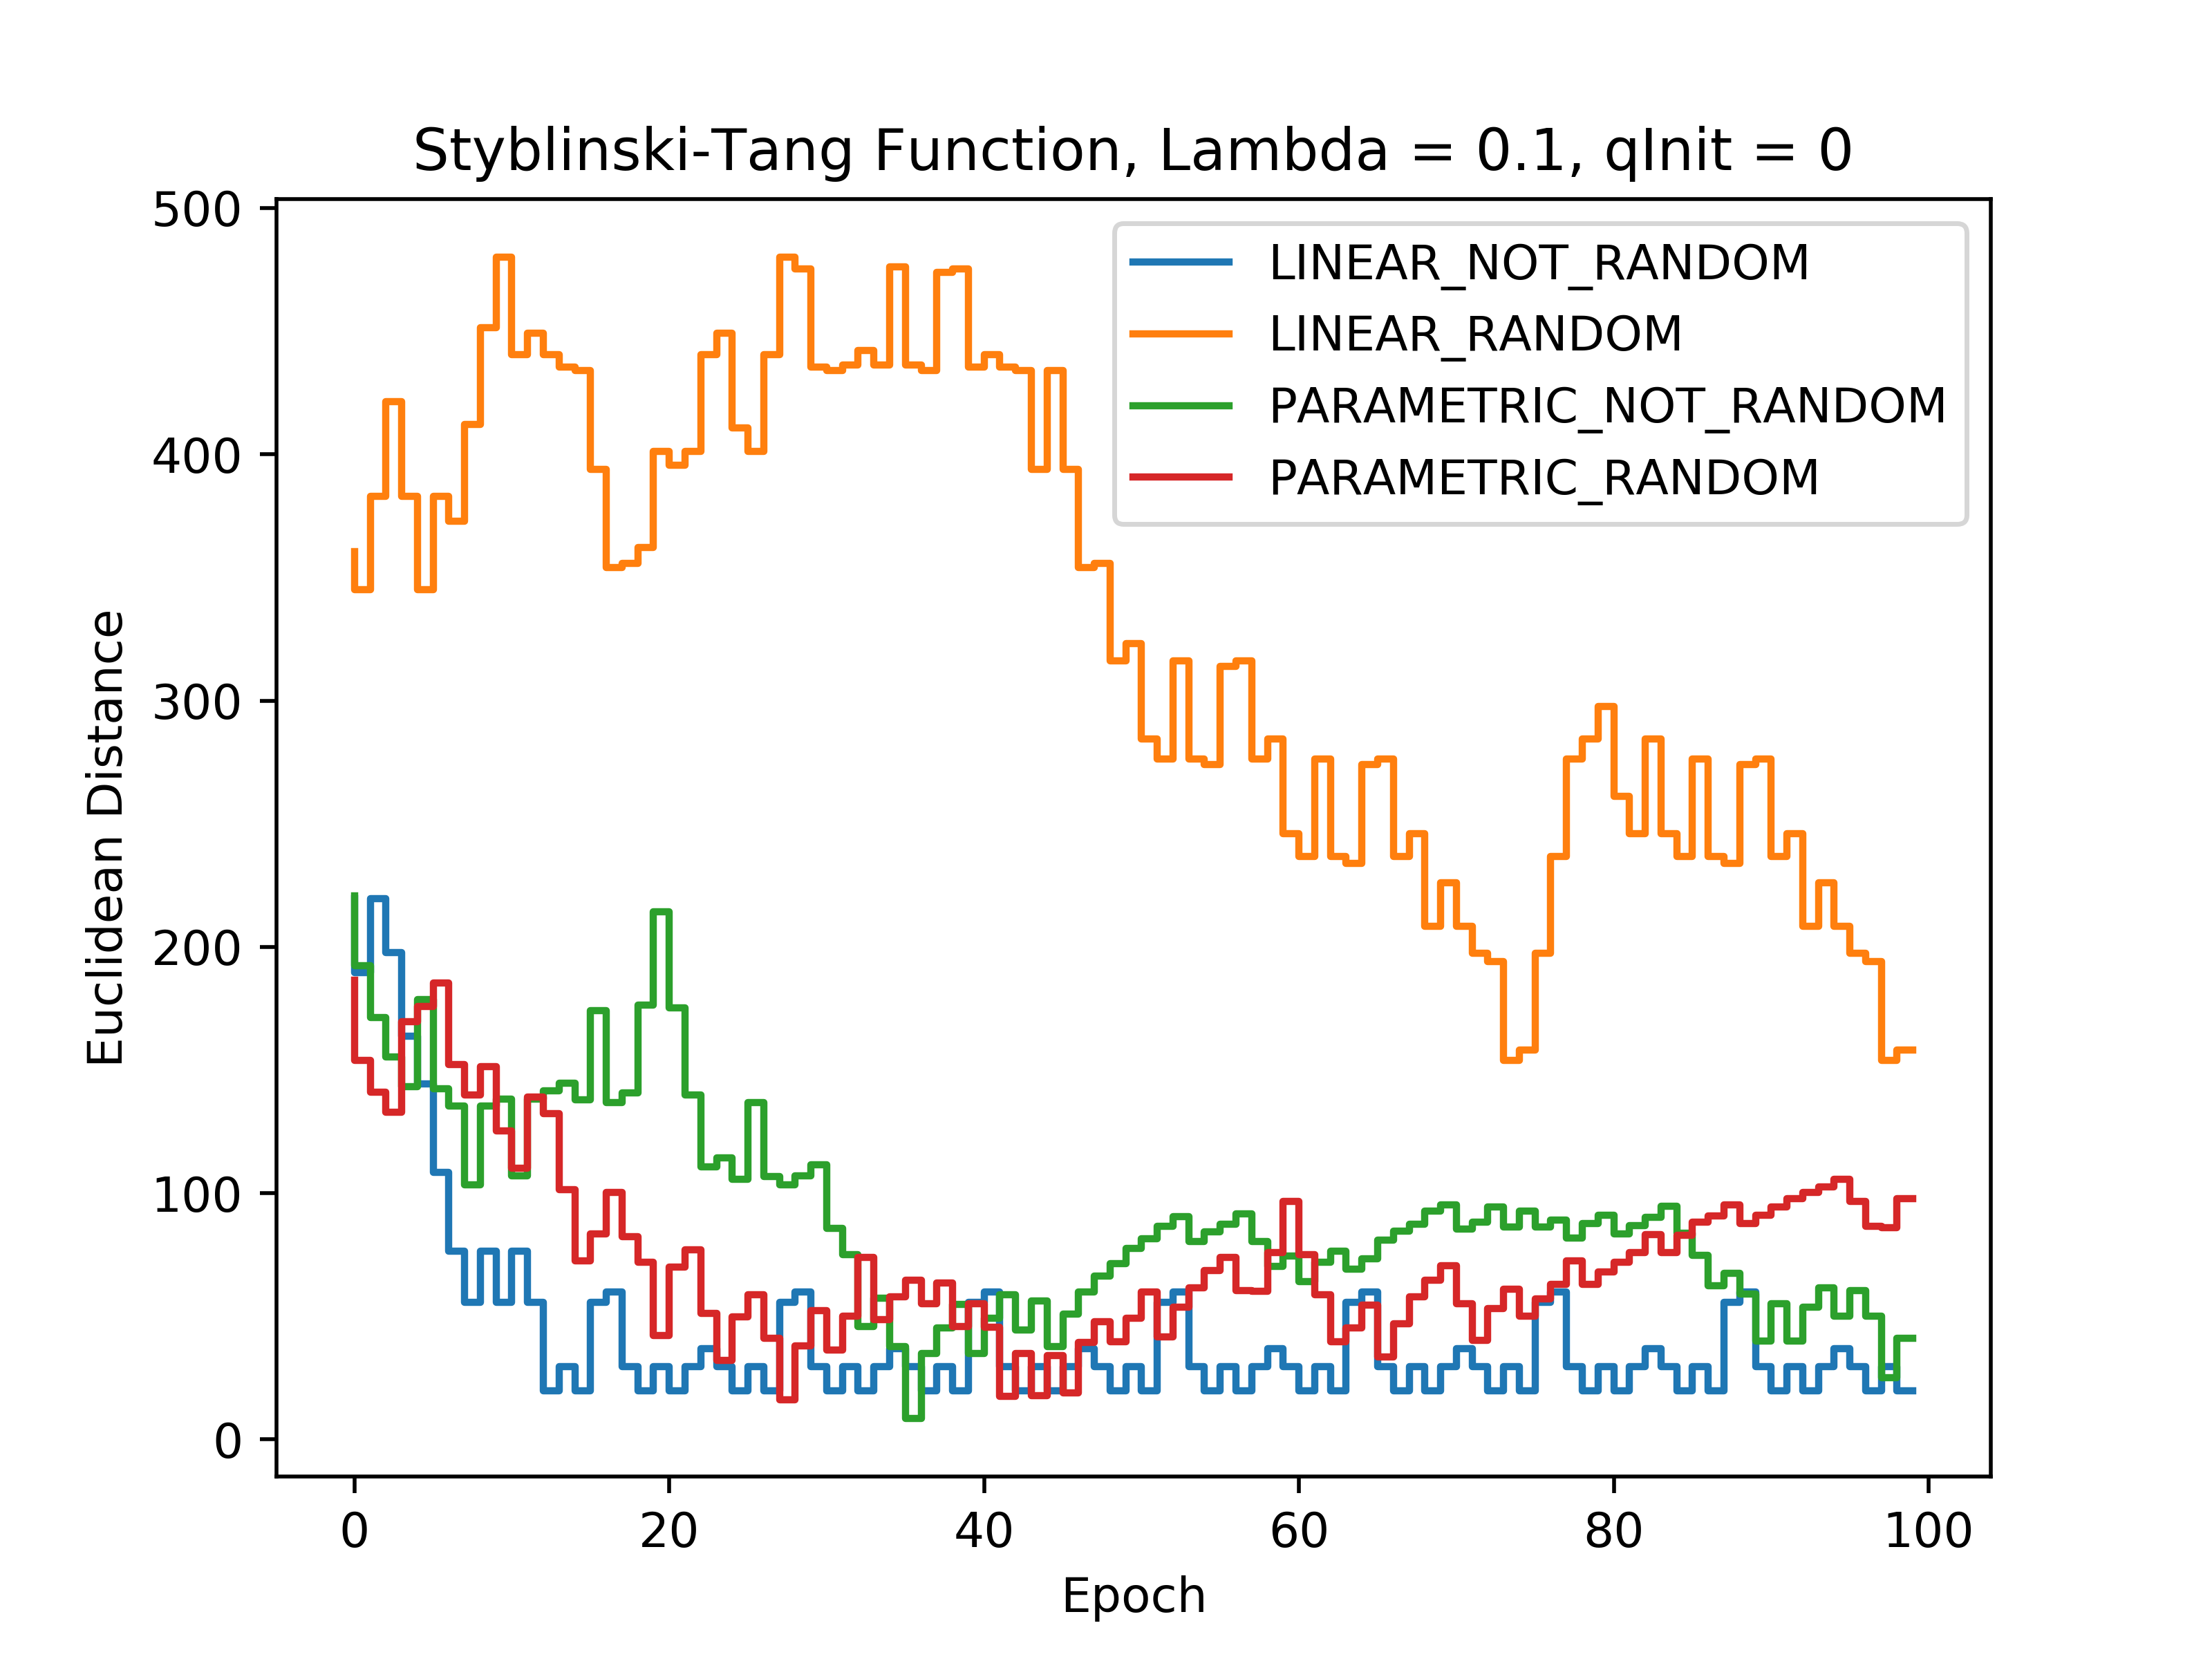
\includegraphics[width=0.4\textwidth]{StyblinskiDifference}
		}
		\subfigure[]{%
			\label{fig:StyblinskiValueFunction}
			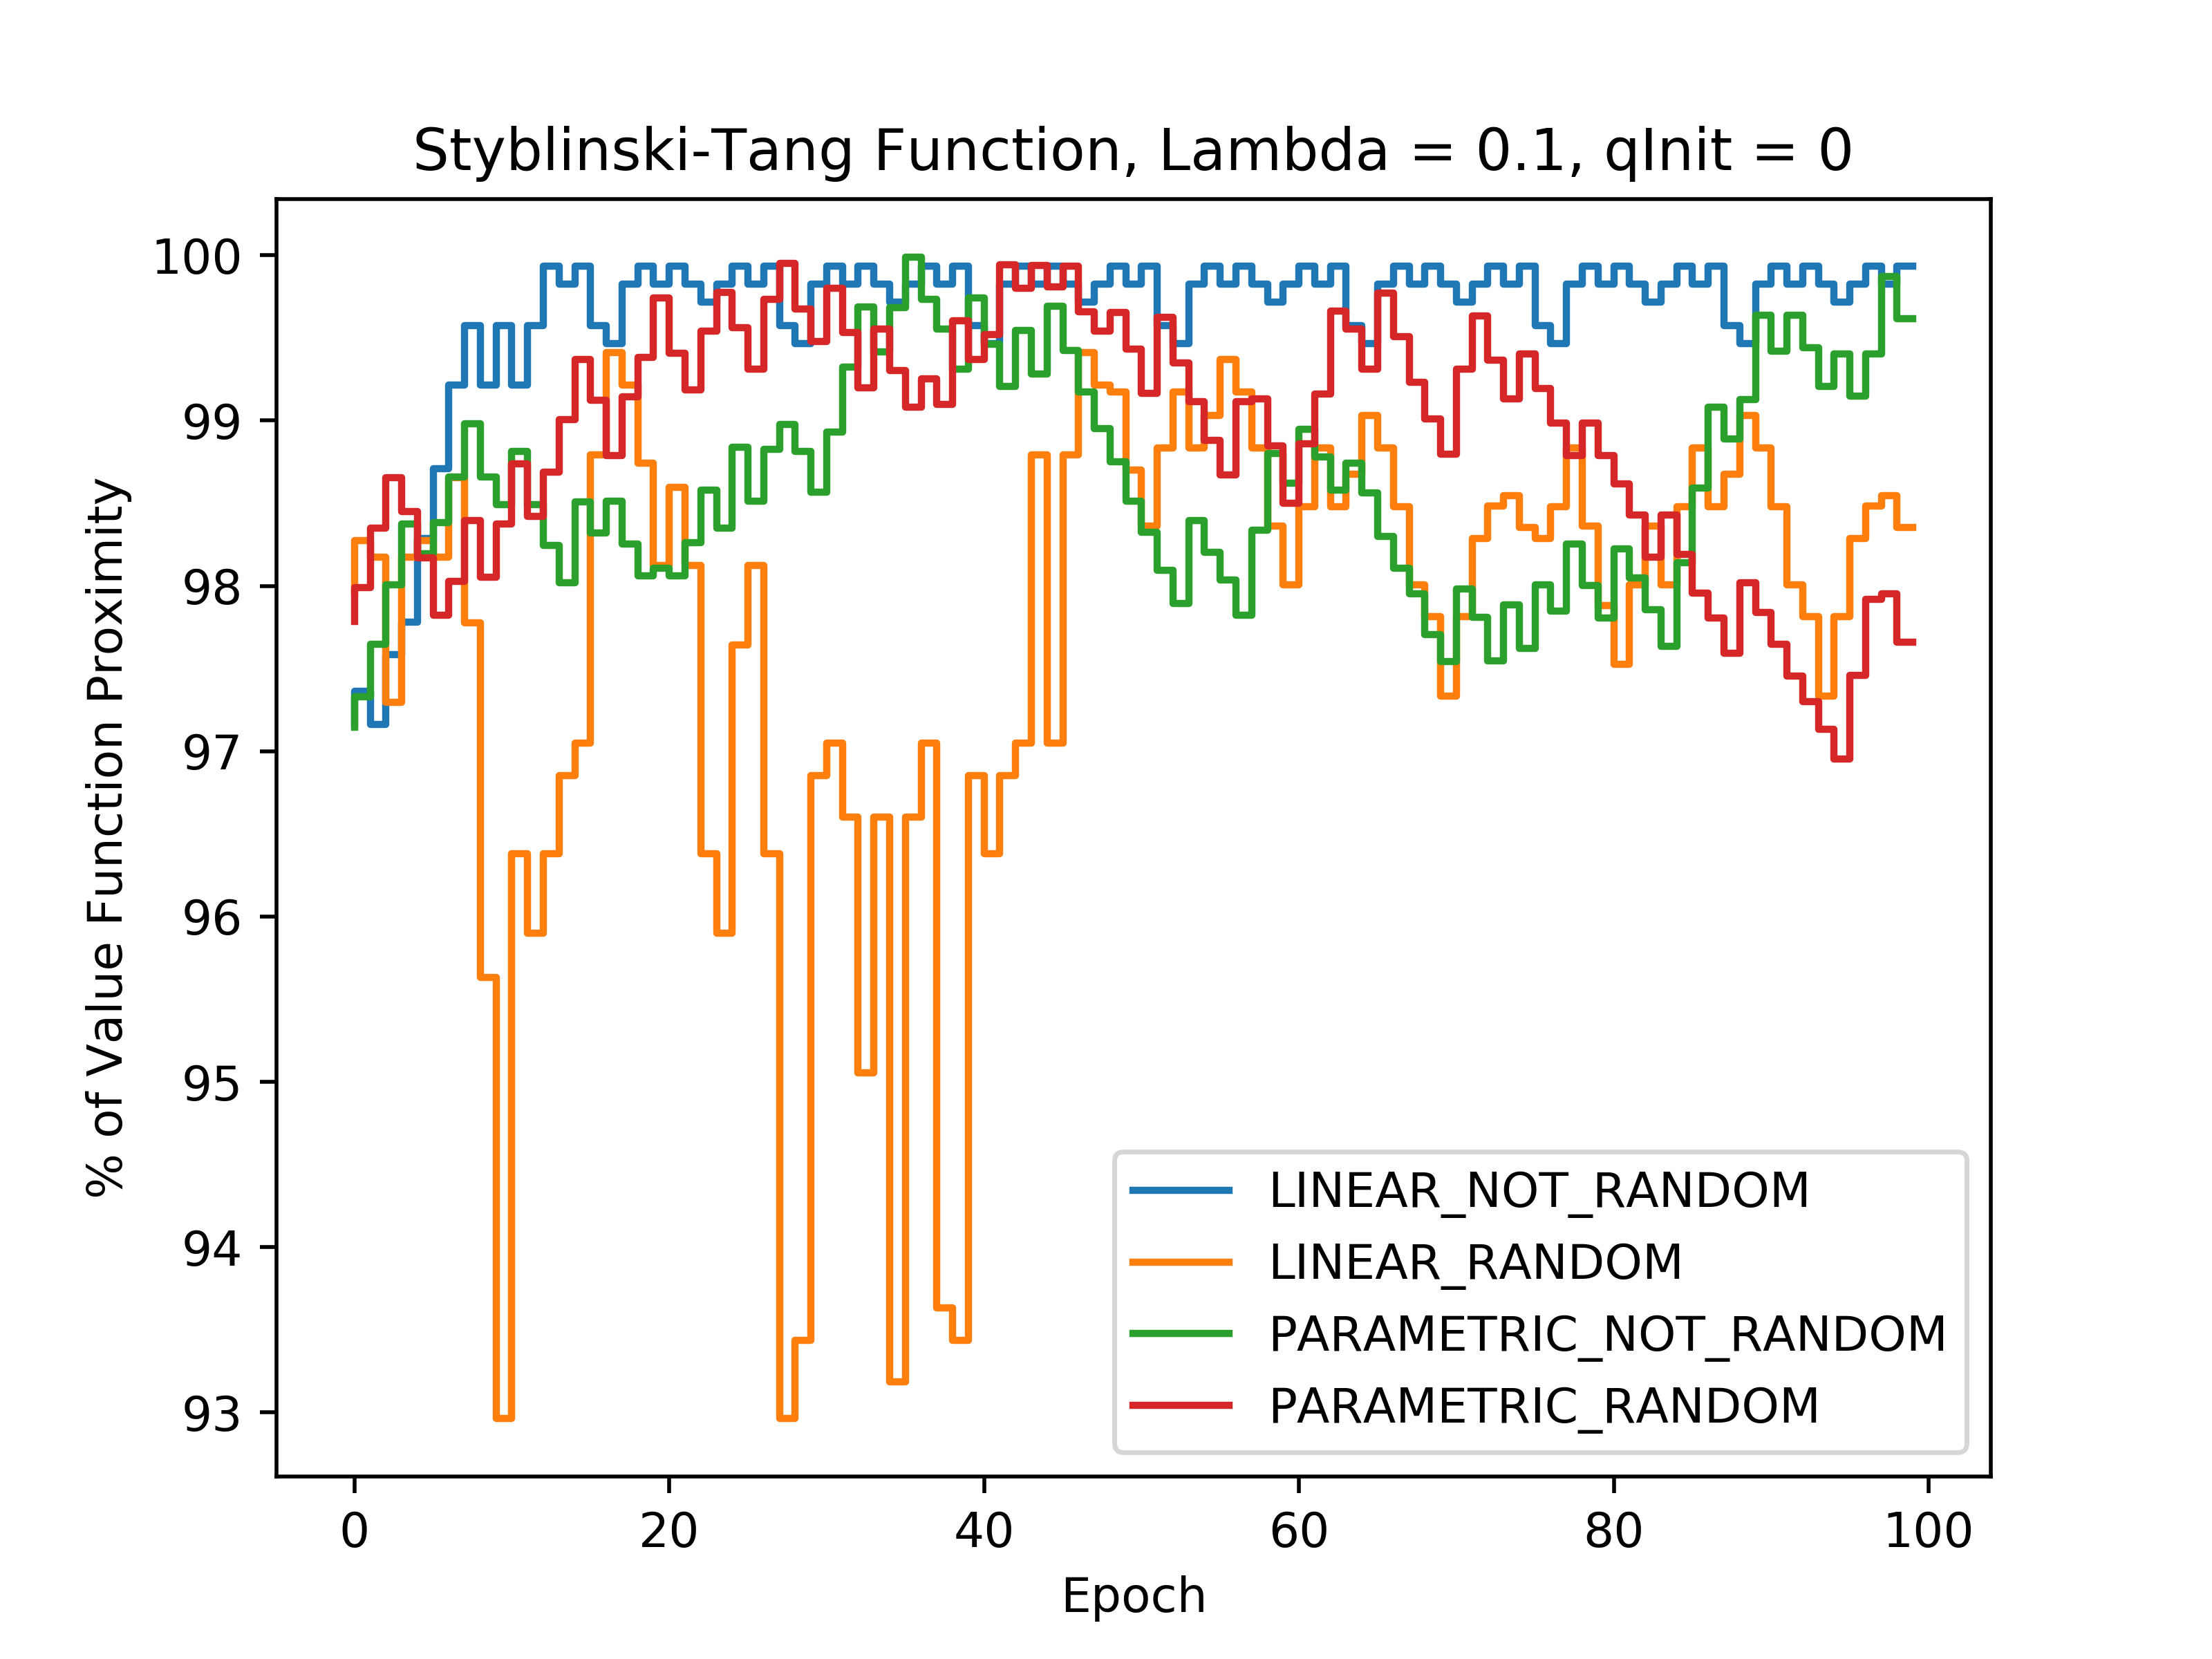
\includegraphics[width=0.4\textwidth]{StyblinskiValueFunction}
		}\\
		\subfigure[]{%
			\label{fig:StyblinskiGap}
			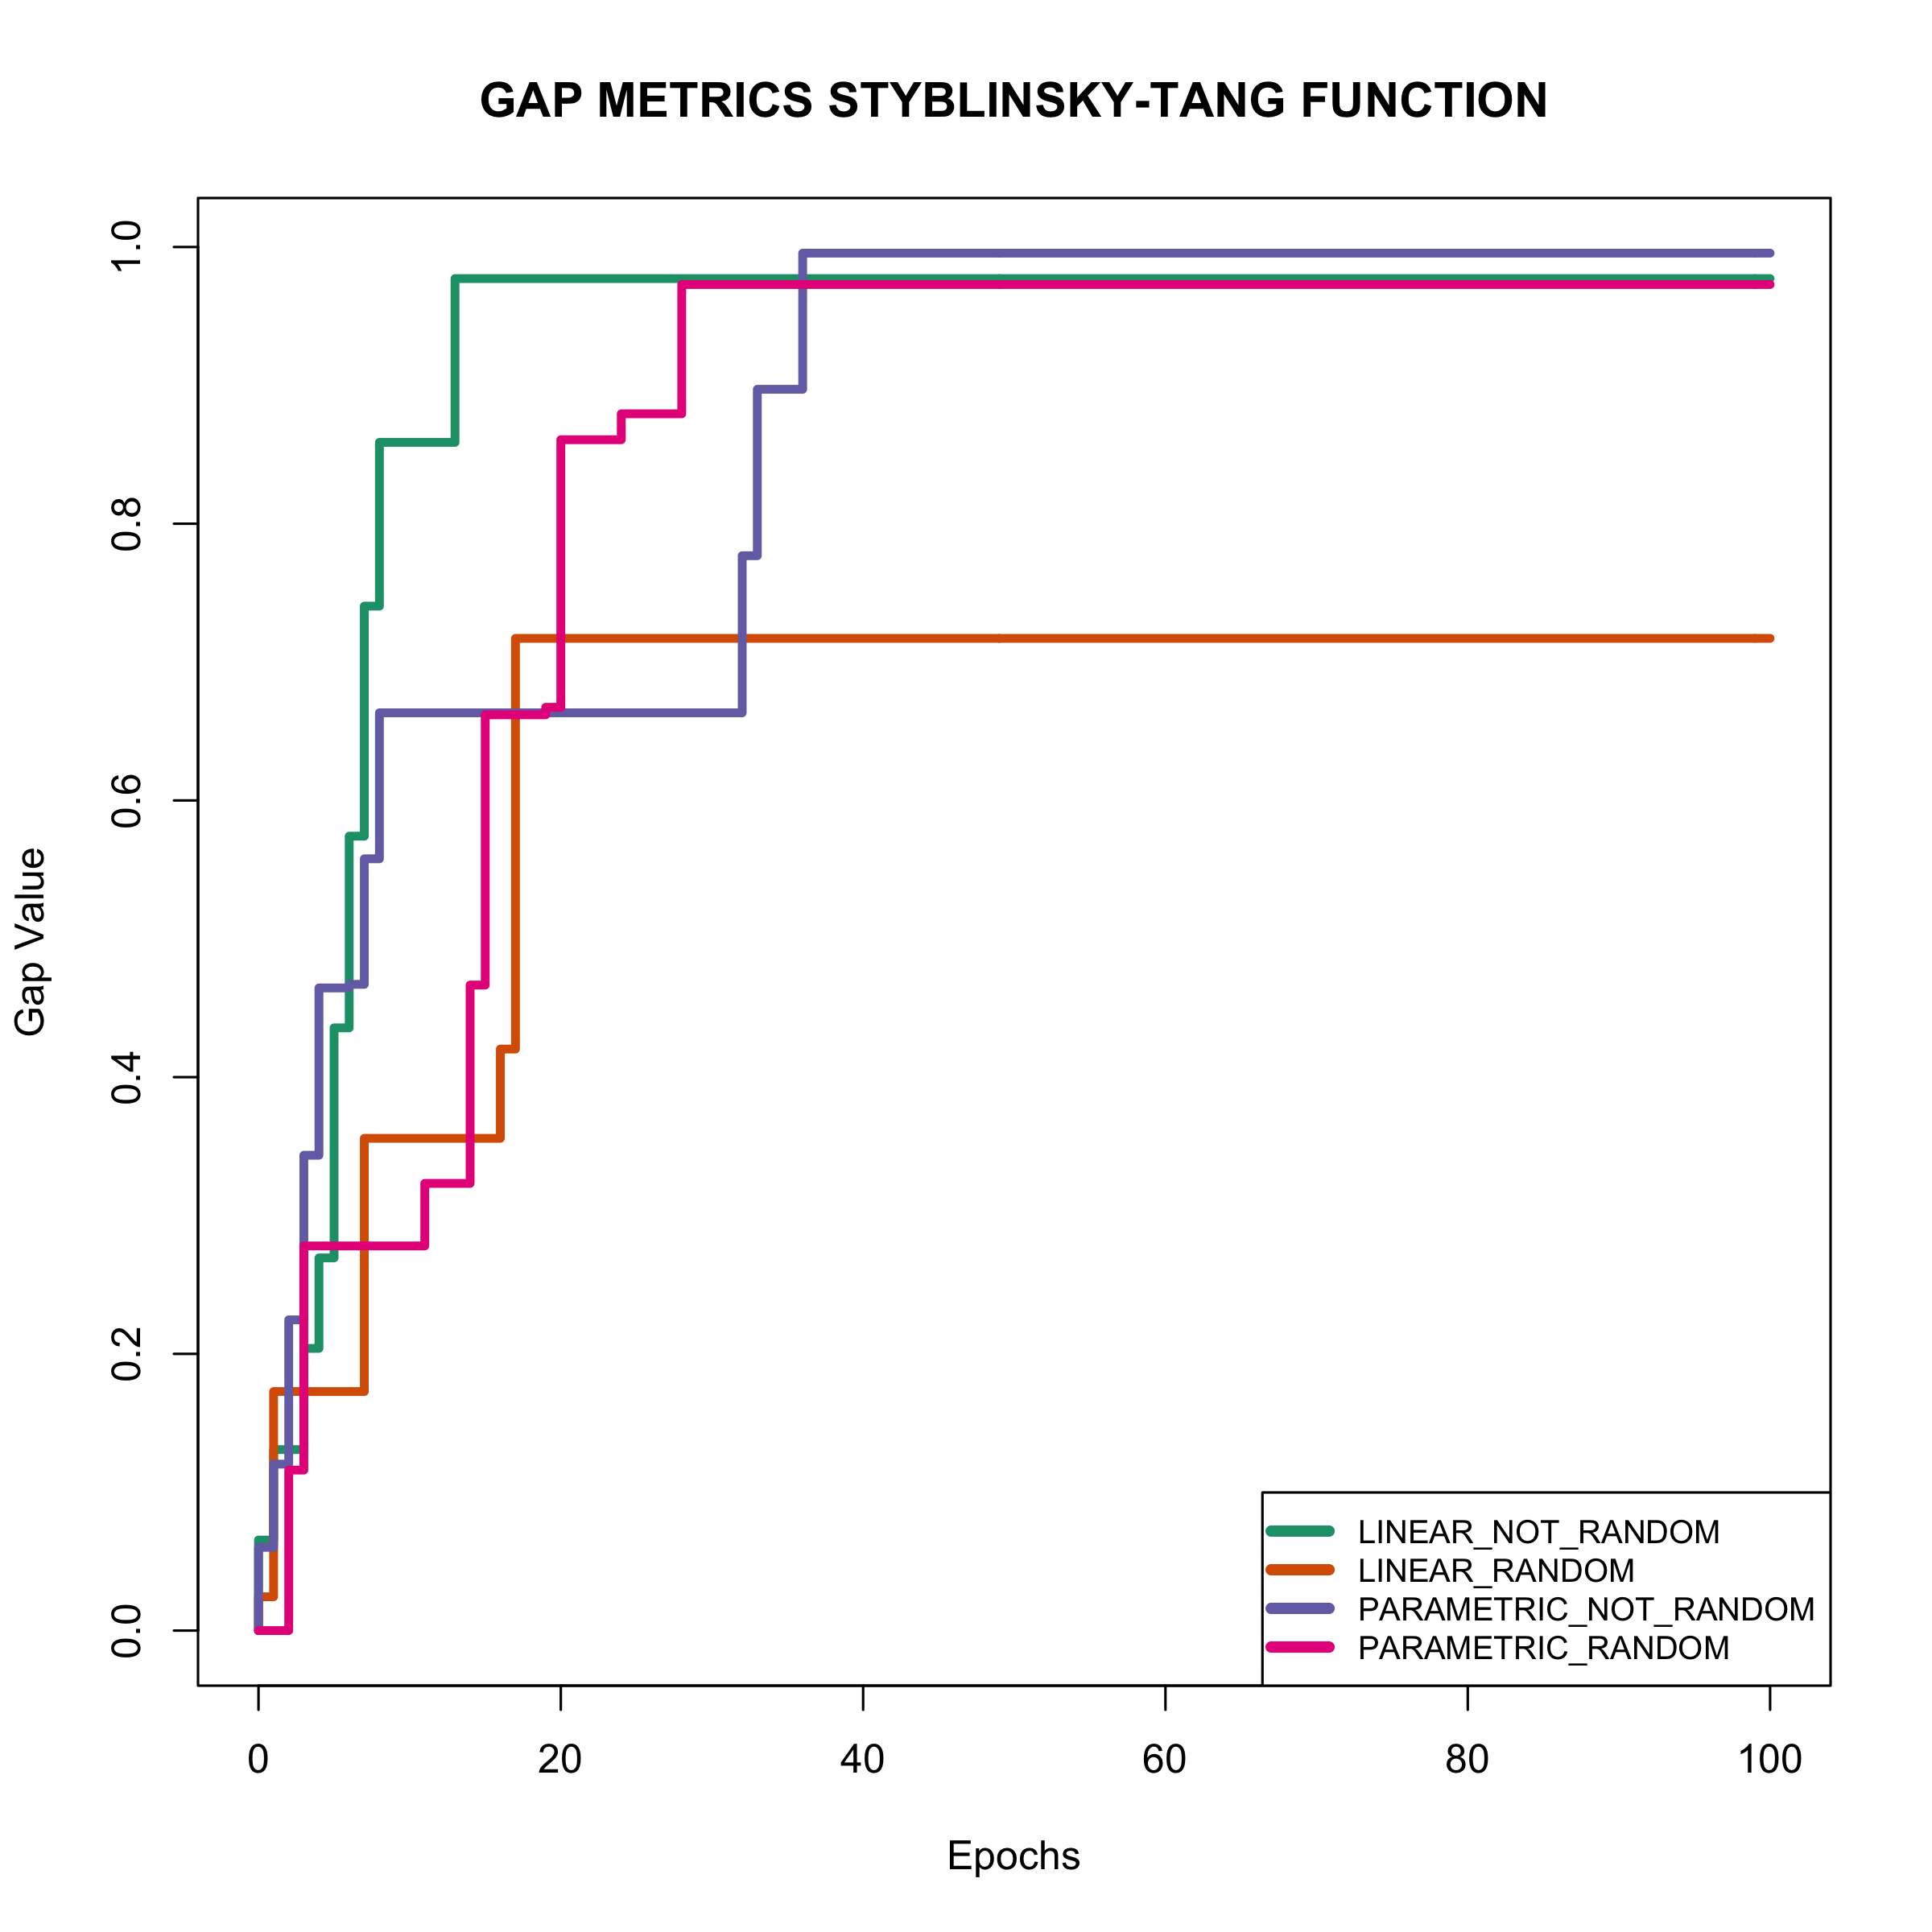
\includegraphics[width=0.4\textwidth]{StyblinskiGap}
		} \\
		
	\end{center}
	\caption{
		Styblinski Function.
	}
	\label{fig:StyblinskiResults}
\end{figure}

\subsection{Styblinski-Tang' s Revised Function} Plot (a) of figure \ref{fig:StyblinskiResults} graphically represents performances of the four possible declinations of {\tt SARSA($\lambda$)} algorithm obtained considering the \textit{Euclidean distance metric}. 

Looking at the {\tt linear, not random} declination's performance, the Euclidean difference between the agent's position and the global maximum is about $200$ pixels. Staring from the twentieth epoch it starts to stabilize around an Euclidean distance level from the maximum of about $40$ pixels. Note that in less than twenty epochs the Euclidean distance from the maximum is about the $20\%$ of the starting one. The current declination also reveals a great stability. With an average Euclidean distance of $43.63$ pixels and a standard deviation of $41.05$, the {\tt linear, not random} declination is the best of the set (table $5.7$).

A decisively worse performance is given by the {\tt linear, random} declination. It starts with an Euclidean distance from the maximum of about $360$ pixels and messily decreases until achieving a level of $180$ pixels. The noise just described is also proved by the highest average Euclidean distance and by the highest standard deviation of the set (table $5.7$).

Last two, parametric declinations give for the first time the possibility to really see behaviour of parametric declination. Starting from about the fiftieth epoch, {\tt parametric, not random} movement starts to imperceptibly increase. This lower amount of movement compared to the non parametric movements depends on the definition of the parametric movement itself. The same behaviour can be seen in {\tt parametric, random} declination starting from epoch $75$. This declination performs better then the {\tt parametric, not random} one in the first epochs but it performs worse in the last ones. With an average Euclidean distance from the maximum of $75.26$ pixels, and with an average standard deviation of $37.34$, the {\tt parametric, random} declinations is generally better than the {\tt parametric, not random} one.

\begin{table}[h!]
	\centering
	\resizebox{\linewidth}{!} {
		\begin{tabular}{c| cccccc} 
			\hline \textbf{Styblinski-Tang Function}
			& \textbf{Mean (pixels)} & \textbf{Standard deviation} \\ 
			\hline Linear not Random
			& \cellcolor{red!25}$43.63$ & \cellcolor{red!25}$41.05$\\ 
			\hline Linear Random
			& $330.16$ & $95.39$ \\ 
			\hline Parametric not Random
			& $91.79$ & $42.24$\\ 
			\hline Parametric Random
			& $75.26$ & $37.34$\\ 
			\hline 
		\end{tabular} 
	}
	\label{StyblinskiTabEuclidean}
	\caption{Euclidean Metric's Performances}
\end{table}

The performance just described is also proved by the percentage of value function' s proximity to the maximum. With an average mean of $99.63\%$ of precision, and a standard deviation of $0.57$, the {\tt linear, not random} declination is the best of the set. General good performances are also made by all other declinations except for the {\tt linear, random} one. Looking at plot (b) of figure \ref{fig:StyblinskiResults} it is possible to note an high instability of this last declination especially until epoch fifty. It than starts to stabilize varying between a proximity level of $97\%$ and $99\%$.

\begin{table}[h!]
	\centering
	\resizebox{\linewidth}{!} {
		\begin{tabular}{c| cccccc} 
			\hline \textbf{Styblinski-Tang Function}
			& \textbf{Mean (\%)} & \textbf{Standard deviation}\\ 
			\hline Linear not Random
			& \cellcolor{green!25}$99.63$ & \cellcolor{green!25}$0.57$ \\ 
			\hline Linear Random
			& $97.73$ & $1.46$ \\ 
			\hline Parametric not Random
			& $98.61$ & $0.66$\\ 
			\hline Parametric Random
			& $98.90$ & $0.74$\\ 
			\hline 
		\end{tabular} 
	}
	\label{StyblinskiTabProximity}
	\caption{Function Proximity in Percentage.} 
\end{table}

Looking at the third plot of figure \ref{fig:StyblinskiResults}, it is possible to note that the best performance is the one of the {\tt parametric, not random} declination. This result obviously depends on the fact that around the thirty-ninth epoch it reaches the maximum for then decisively distance itself from it. This behaviour is again due to the absence of an adequate training space. This lack prevents the agent from developing an optimal policy.

\begin{sidewaystable} 
	\centering
	\label{table:BestSoundings}
	\caption{Best Soundings}
	\begin{tabular}
		{l l l l l} \hline Name & Linear Not Random & Linear Random & Parametric Not Random & Parametric Random \\
		\hline Himmelblau & \vtop{\hbox{\strut $2486.938$}\hbox{\strut $(2.67, 1.34)$}\hbox{\strut}\hbox{\strut}} &\cellcolor{blue!25} \vtop{\hbox{\strut $2498.457$}\hbox{\strut $(3.67, -1.57)$}\hbox{\strut}\hbox{\strut}} & \vtop{\hbox{\strut $2485.972$}\hbox{\strut $(-2.1, 3.30)$}\hbox{\strut}\hbox{\strut}} & \vtop{\hbox{\strut $2492.11$}\hbox{\strut $(-2.283, 3.234)$}\hbox{\strut}\hbox{\strut}} \\
		Sphere & \vtop{\hbox{\strut $3484.44$}\hbox{\strut $(-8.8, -0.67)$}\hbox{\strut}\hbox{\strut}} & \vtop{\hbox{\strut $3537.986$}\hbox{\strut $(-3.24, 3.40)$}\hbox{\strut}\hbox{\strut}} &\cellcolor{blue!25} \vtop{\hbox{\strut $3557.722$}\hbox{\strut $(-1.034, -1.099)$}\hbox{\strut}\hbox{\strut}} & \vtop{\hbox{\strut $3553.626$}\hbox{\strut $(1.69, 1.88)$}\hbox{\strut}\hbox{\strut}} \\
		Beale & \vtop{\hbox{\strut $1985.797$}\hbox{\strut $(0, 0)$}\hbox{\strut}\hbox{\strut}} & \vtop{\hbox{\strut $1472.184$}\hbox{\strut $(1.69, 2.269)$}\hbox{\strut}\hbox{\strut}} &\cellcolor{blue!25} \vtop{\hbox{\strut $1997.392$}\hbox{\strut $(-0.77, 1.559)$}\hbox{\strut}\hbox{\strut}} & \vtop{\hbox{\strut $1994.983$}\hbox{\strut $(1.309, -0.89)$}\hbox{\strut}\hbox{\strut}} \\
		Styblinski-Tang & \vtop{\hbox{\strut $5153.086$}\hbox{\strut $(-2.67, -2.67)$}\hbox{\strut}\hbox{\strut}} & \vtop{\hbox{\strut $5126.192$}\hbox{\strut $(3, -2.97)$}\hbox{\strut}\hbox{\strut}} &\cellcolor{blue!25} \vtop{\hbox{\strut $5155.97$}\hbox{\strut $(-2.77, -2.95)$}\hbox{\strut}\hbox{\strut}} & \vtop{\hbox{\strut $5154.053$}\hbox{\strut $(-3.17, -2.99)$}\hbox{\strut}\hbox{\strut}} \\
		\hline
	\end{tabular}
\end{sidewaystable}

\section{ \enquote{Experienced} SARSA($\lambda$) Algorithm}

In the previous section, performances of SARSA($\lambda$) algorithm on single test functions have been analysed. In this section a different experiment on SARSA($\lambda$) algorithm is described. For each declination, the algorithm has been trained according to the unique, previously described configuration on Himmelblau's Function, Sphere Function, Beale Function. At the beginning of each training, except for the Himmelblau's Function's one, for each different declination, the {\tt qTable} obtained from previous trainings on previous functions, has been loaded and updated. The agent was finally executed on Styblinski-Tang' s Revised Function, only using the greedy configuration. It is possible to resume what just said as shown in algorithm \ref{ExpertAlgo}.

\begin{algorithm} [h!]

\For {given configurations} {
	\For {each declination}
	{execute on Himmelblau's Function; \\
		write {\tt qTable} for Himmelblau's Function's execution; \\
		load {\tt qTable}; \\
		execute on Sphere Function; \\
		update {\tt qTable}; \\
		load {\tt qTable}; \\
		execute on Beale Function; \\
		update {\tt qTable}; \\
		load {\tt qTable}; \\
		execute only greedy episode for Styblinski-Tang Revised Function;
	} 
}
	\caption{"Expert" Sarsa($\lambda$) Algorithm} 
	\label{ExpertAlgo}
\end{algorithm}

\begin{figure} [h!]
	\centering
	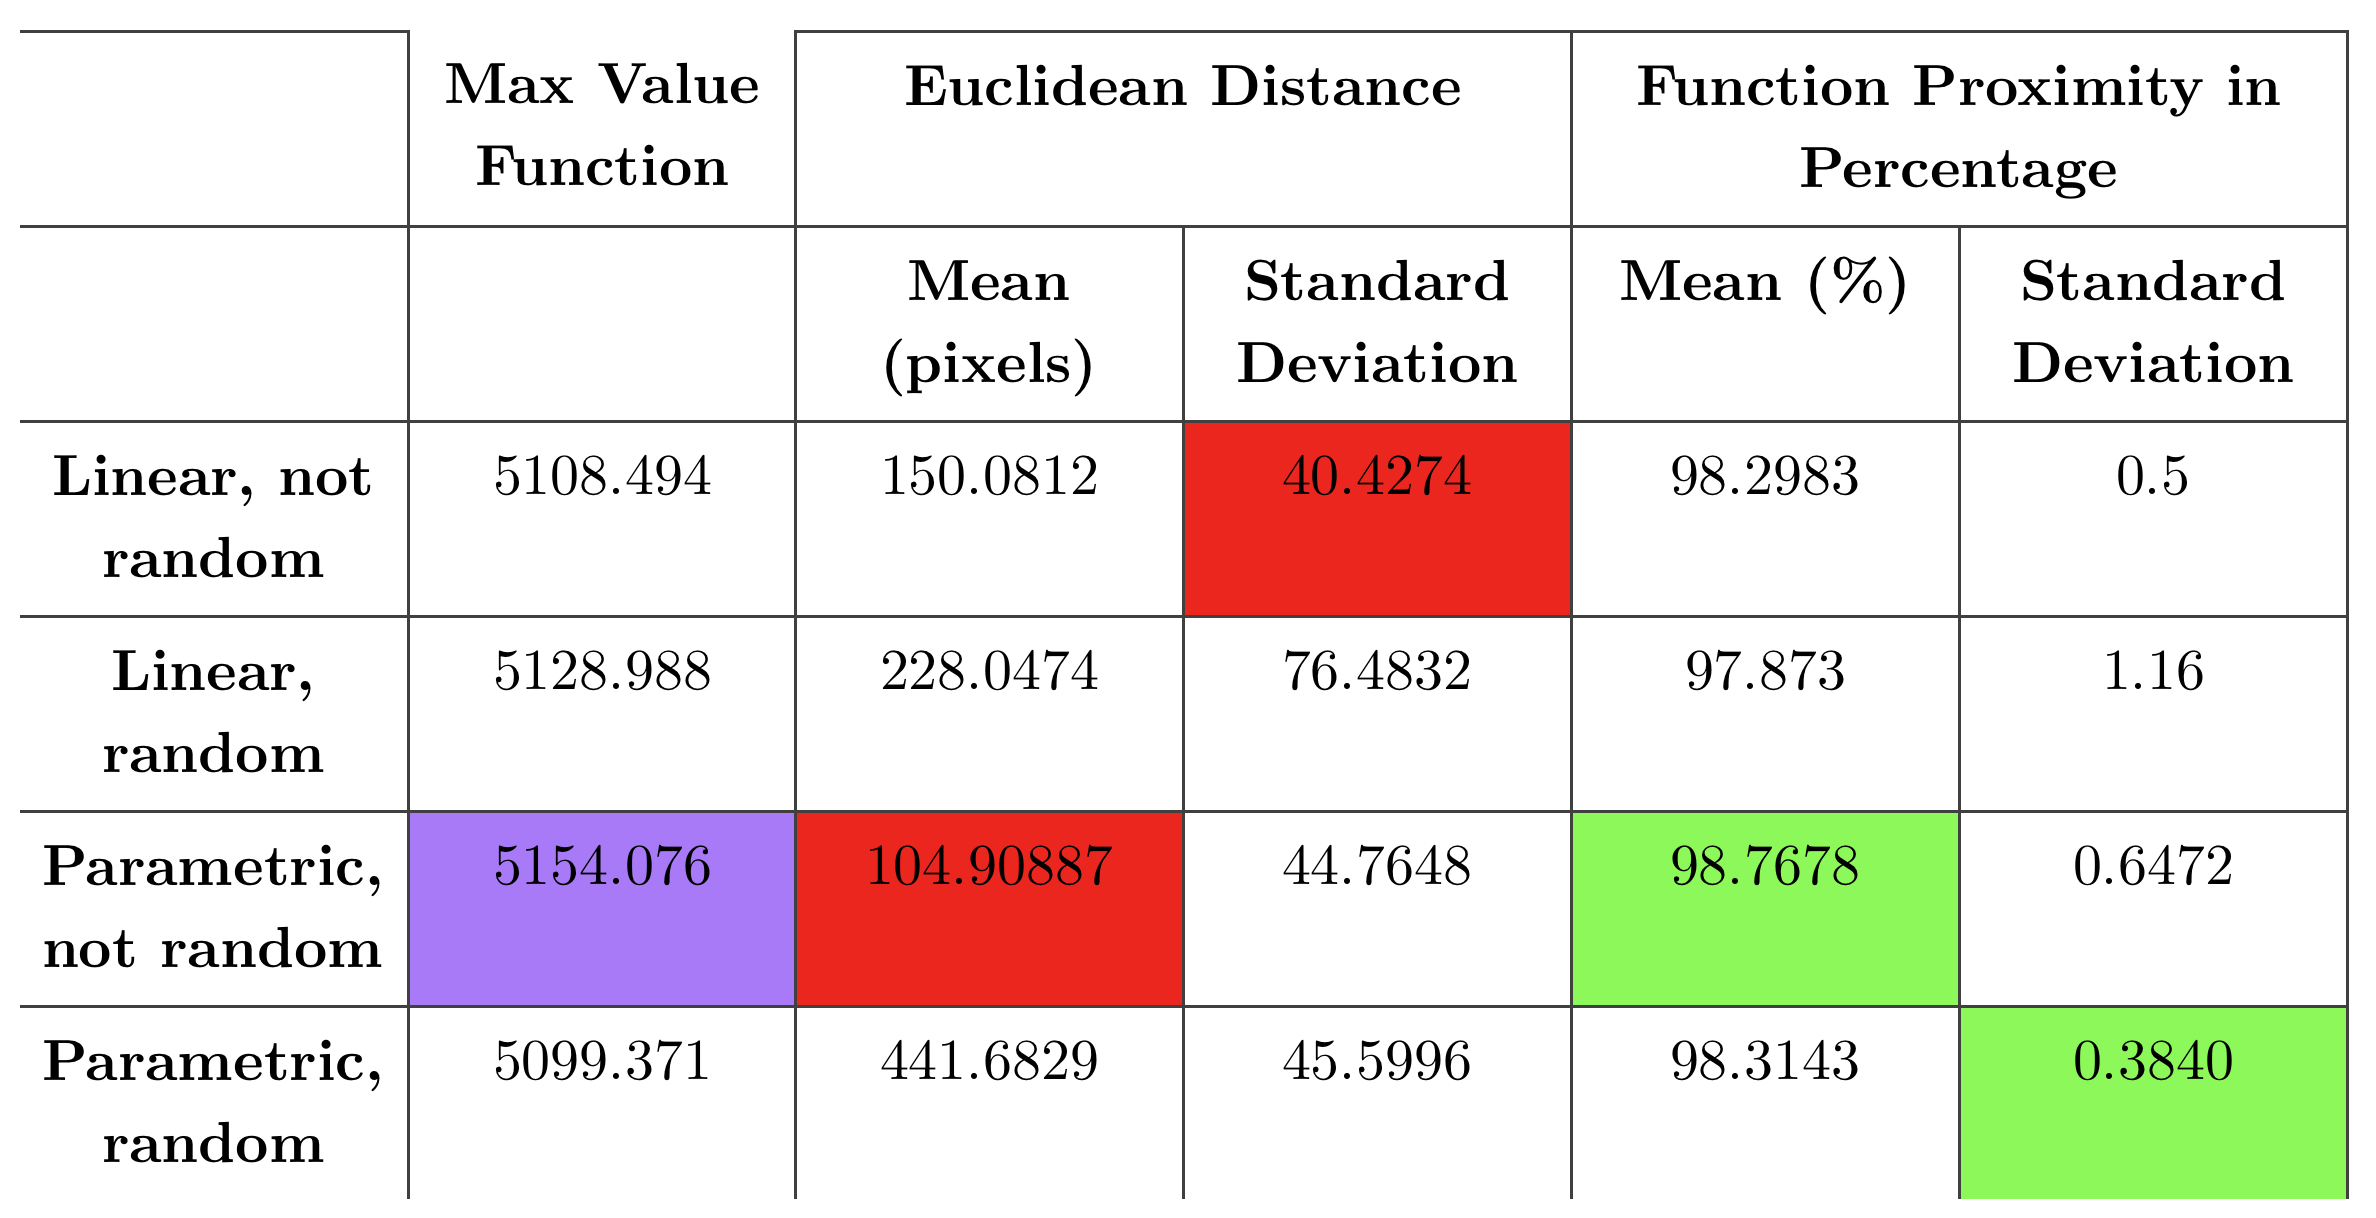
\includegraphics[width=\linewidth]{IMAGES/ExpertReasumingTable}
	\caption{Expert Sarsa($\lambda$)'s Performances Table}
	\label{fig:expertreasumingtable}
\end{figure}
 
The goal of this experiment is to measure how much the \textit{previously acquired experience} from training on different functions, is useful in maximizing a new, never tested before black-box function.

\begin{figure}[h!]
	\begin{center}
		\subfigure[]{%
			\label{fig:StyblinskiDifference}
			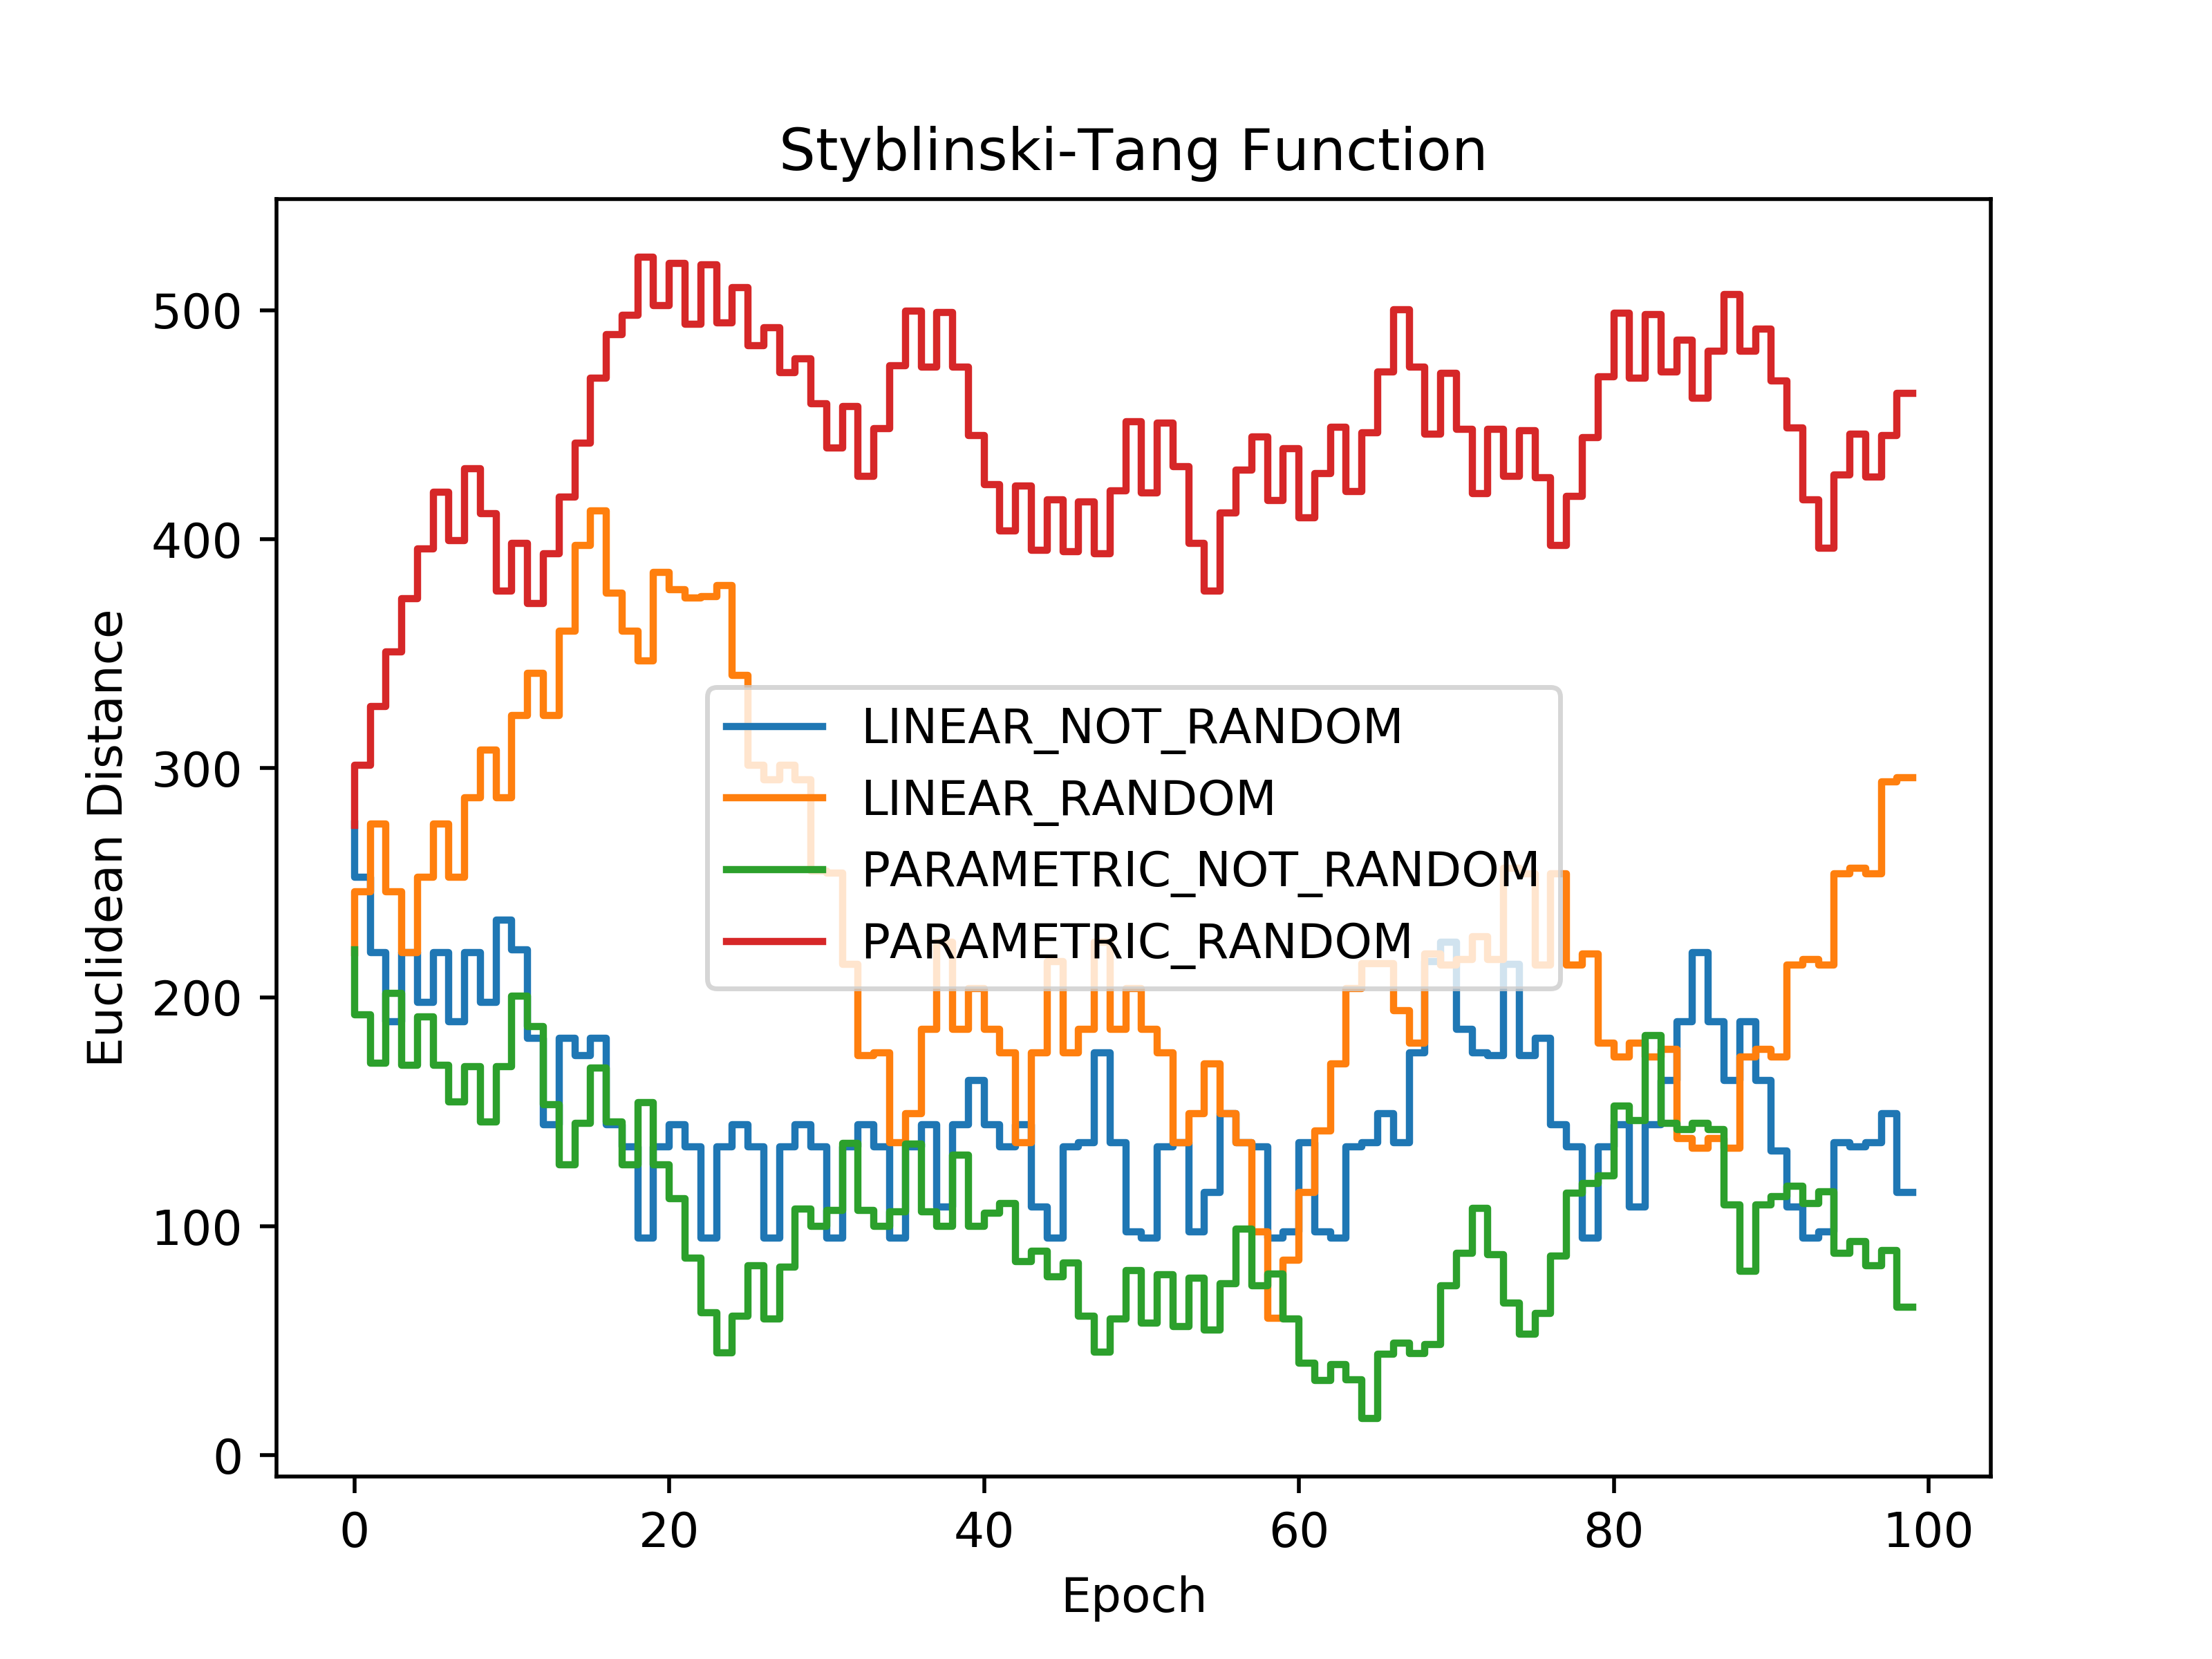
\includegraphics[width=0.4\textwidth]{ExpertStyblinskiDifference}
		}
		\subfigure[]{%
			\label{fig:StyblinskiValueFunction}
			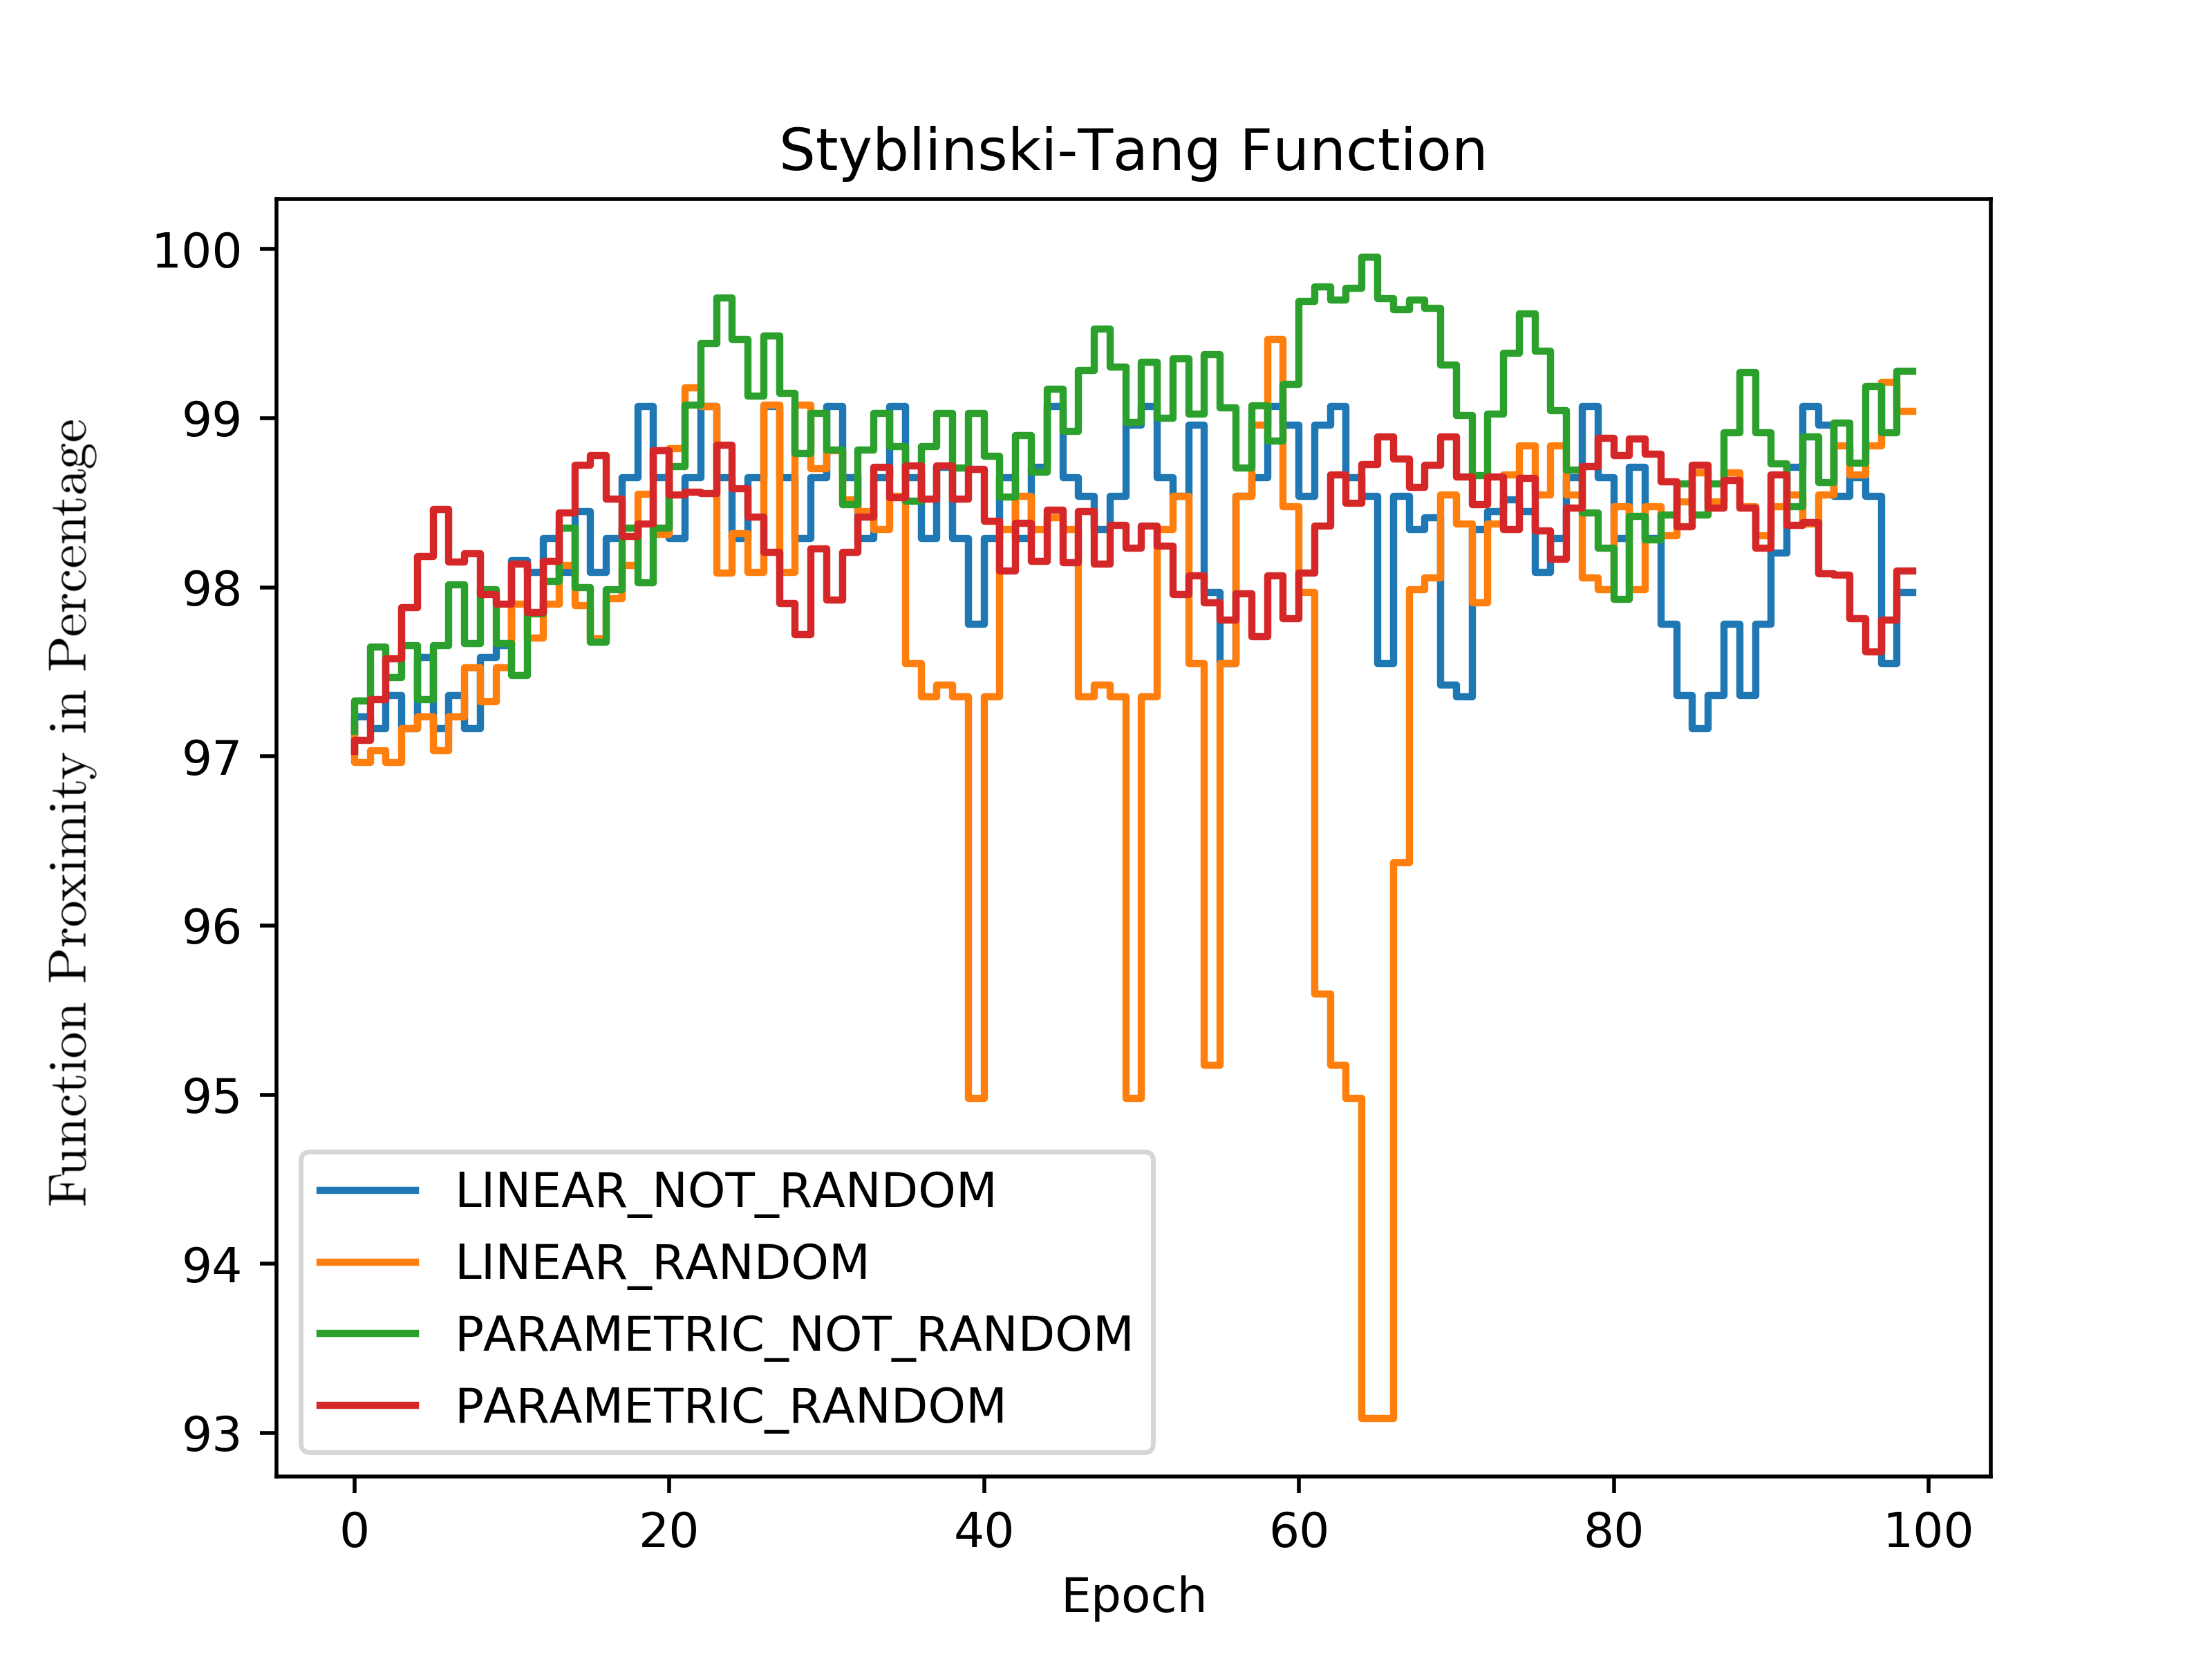
\includegraphics[width=0.4\textwidth]{ExpertStyblinskiValueFunction}
		}\\
		\subfigure[]{%
			\label{fig:StyblinskiGap}
			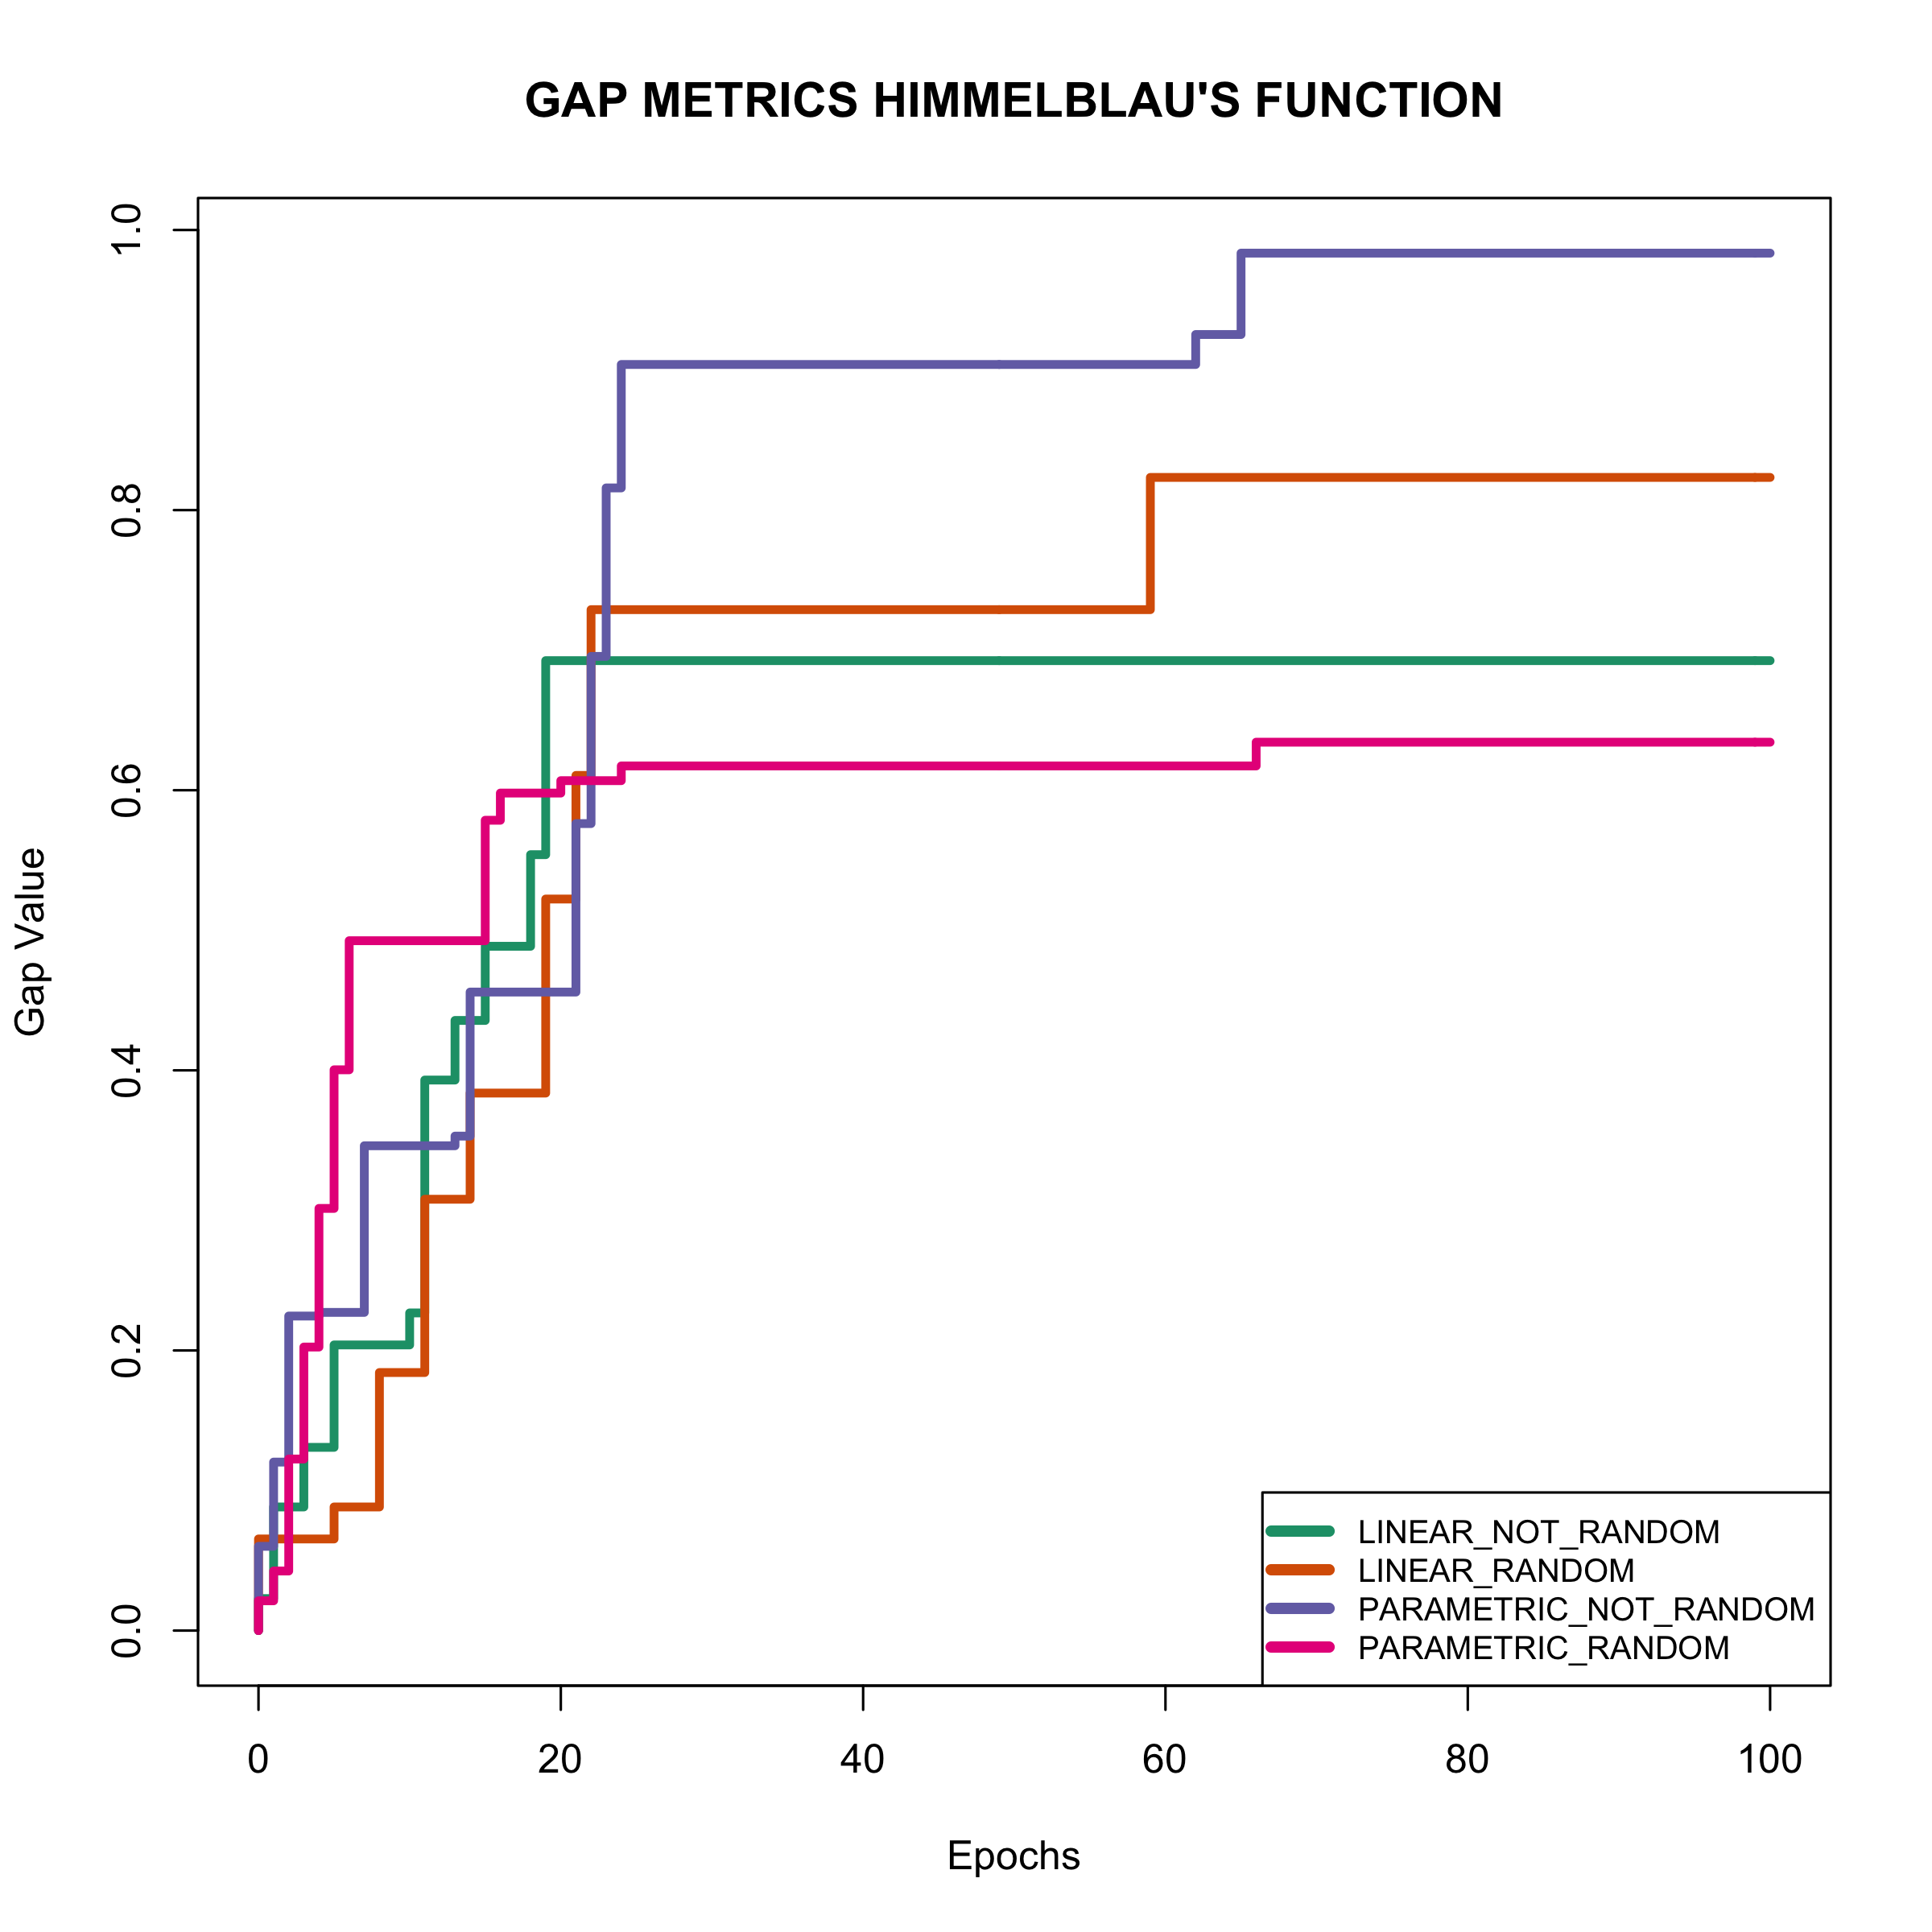
\includegraphics[width=0.4\textwidth]{ExpertGap}
		} \\
		
	\end{center}
	\caption{
		"Expert" SARSA($\lambda$)'s  performances.
	}
	\label{fig:ExpertResults}
\end{figure}

Looking at plot (a) of figure \ref{fig:ExpertResults} it is immediately possible to note that the richest previously acquired experience is given by the {\tt parametric, not random} configuration. In this case, the previously acquired experience on previously tested functions is well expendable with unknown functions. The average Euclidean distance from the maximum in the greedy episode, executed on the never tested function, is equal to $104.90887$ pixels. Despite of this positive value, it is also important to underline the high instability in the same measure. The standard deviation is equal to $44.7648$. The average percentage of value function's proximity to the maximum, is  equal to $98.7678\%$ with a standard deviation of $0.6472$. The general good performance of this declination is confirmed by the fact that the {\tt Gap Value} is the highest between the considered declinations of the employed configuration (plot (c) of figure \ref{fig:ExpertResults}). 

The less reach previously acquired experience is guaranteed by the {\tt parametric, random} configuration. In this case, the Euclidean distance from the maximum constantly swings between $400$ and $500$ pixels. The average Euclidean distance is $441.6829$ pixels with a greater instability certified by the high average standard deviation ($45.5996$) of this measure. Despite of those bad values, it is important to underline that the average percentage of value function's proximity to the maximum is equal to $98.3243\%$ with the lowest standard deviation, which is equal to $0.384$. The general bad performance of this declination is also certified by the lowest {\tt Gap Value} which is equal to $0.6$.

In general, it is possible to say that the two declinations able to guarantee an adequate previously acquired experience useful to maximize black-box, never tested before functions, only running the greedy episode, are the {\tt parametric, not random} declination and the {\tt linear, not random} declination. It is interesting to note that they are both {\tt non random} declinations. It clearly depends on the location of the random starting points during the training phase. Changing the selected seed, those declinations could give better performances.

\section{Humans' Optimization Strategies}

In order to study humans' strategies in the optimization of black-box functions, three acquisition functions are considered :

\begin{itemize}
	\item Upper Confidence Bound ({\tt UCB}) \cite{DBLP:journals/pieee/ShahriariSWAF16}
	\item Probability of Improvement ({\tt PoI}) \cite{DBLP:journals/pieee/ShahriariSWAF16}
	\item Expected Improvement ({\tt EI}) \cite{DBLP:journals/pieee/ShahriariSWAF16}
\end{itemize}

In addition to acquisition functions, also the GP is represented. \\ 

\begin{figure} [h!]
	\centering
	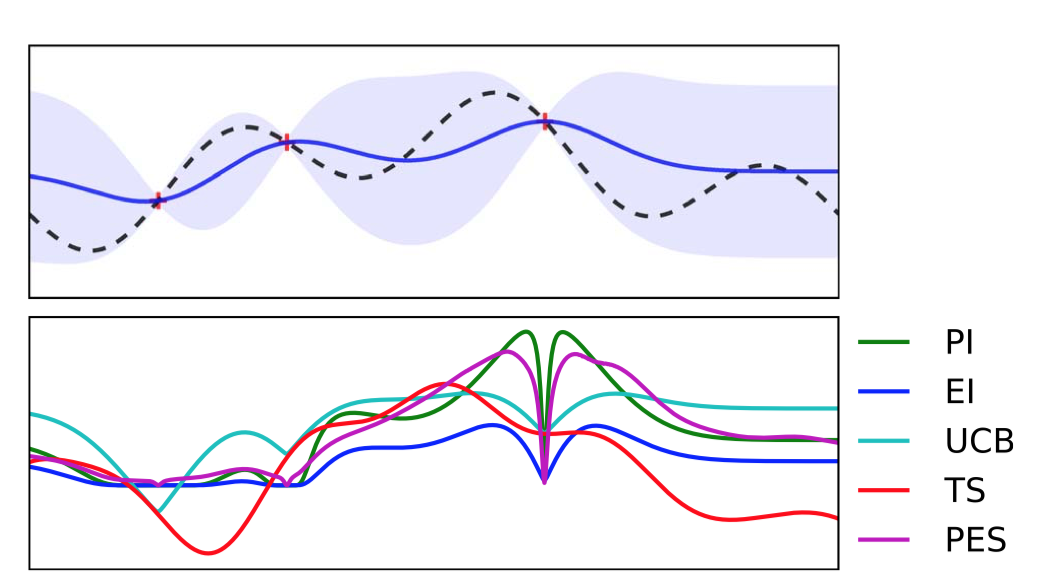
\includegraphics[width=\linewidth]{IMAGES/Surrogate}
	\caption{An example of a GP and associated acquisition functions.}
	\label{fig:surrogate}
\end{figure}

Only the best player's first performance for each function is considered. This means that even if each player has had three possibilities, each one composed of fifteen attempts, for each function (except for the Styblinski-Tang Revised function), only the first one of the three rounds made by the best player for the function itself is here considered. This choice is made in order to study humans' behaviour in the case of no previously experience of the specific function to optimize. The best player is selected according to the highest score reached for each function. In the case there were two best players, the first one's performance is considered.  \\

Results obtained for each function can be found at this link \footnote{\url{https://github.com/AntonioBr/IMAGES/tree/master/HUMANS}} . For each function,  for all the fifteen attempts considered, the first three attempts are employed in order to create the original GP. Starting from the fourth attempt, the white star is employed in order to underline the new attempt chosen by the human compared to the "best" one proposed by the various acquisition functions. Other black points represent previously made attempts. Comparing choices made by human and acquisition functions, it will be clear which one of considered acquisition functions, has led the human in his/her choices.

\subsection{Himmelblau Function}
In the case of the Himmelblau's Function the best player maximizes according to no one on the considered acquisition functions. Looking at the sequence of attempts, the player seems to choose a radically, exploratory approach. All acquisition functions, instead, present a balanced explorative-exploitative approach based on observed data. Looking at the GP obtained at the fifteen attempt, it is possible to note that the original, black-box function is well approximated.

\subsection{Sphere Function}
In the case of the Sphere Function the best player maximizes according to {\tt PoI} acquisition function. The process to achieve the maximum is linear and the player never try a radical different exploratory attempt. The GP well approximates the real, black-box function still starting from the sixtieth attempt.

\subsection{Beale Function}
In the case of the Beale Function the best player maximizes according to {\tt PoI} acquisition function until the sixtieth attempt. Starting from the seventh attempt it maximizes according to {\tt UCB} acquisition function till the fifteenth attempt. After fifteen attempts, the GP does not well approximate the real, hidden function, but isolates the region of the maximum.

\subsection{Styblinski Revised Function}
The case of the Styblinski revised function is surely the most interesting one. By default, the best player can make only one round composed by fifteen attempts. The best player is here defined just according to its only, experience-free set of attempts. In this case the best player maximizes according to the {\tt UCB} acquisition function. Also in this case, after fifteen attempts the GP does not well approximate the real, black-box function, but isolates the region of the maximum. This means that the player did not make enough exploration. It is interesting to note how it is possible to identify an acquisition function corresponding to the human reasoning process, considering that it was not possible in the case of the Himmelblau's Function. It is also interesting to note how the best player in this case is different from the one of the Himmelblau Function. The two functions were selected because of their shapes' similarity. Results obtained are different for the two similar functions. \\

In the $100\%$ of cases, best players are male. Their mathematical knowledge level is in the $100\%$ of cases the highest possible. They are all test subjects with an age between $19$ and $22$.

\section{RL Agent's  policy vs Humans' Strategies}
All experiments described in the previous sections are useful to better understand the one described in the current section. As previously said, one of the main goals of this thesis is comparing humans' strategies with the policy adopted by a RL agent in the optimization of black-box $2d$-functions. In order to do this, it has been considered the case of maximization of Styblinski-Tang' s Revised Function. In the previous section, humans' strategy with no previously acquired knowledge about a specific function, has been studied. Making the same study on performances of a RL agent could be not very fruitful because of the great amount of training required by the algorithm in order to obtain acceptable results. Despite of this, a good choice is to compare humans' performances and RL agent's ones in the case of maximization of black-box $2d$-functions with \textit{previously acquired experience}. To be more specific, when one of the human test subjects, maximizes the Styblinski-Tang's Revised Function, he/she has already had experience with optimization of Himmelblau's Function, Sphere Function, Beale Function. The same is for the RL agent in the case of the \enquote{Experienced} SARSA($\lambda$) algorithm.

In the human case, the best player optimizes according to the {\tt UCB} acquisition function. After fifteen attempts the GP does not well approximate the real, black-box function, but isolates the region of the maximum. The case of RL agent is more complex. As seen in the plots of figure \ref{fig:ExpertResults}, the {\tt parametric, not random} declination is the one with the best performances. The RL agent which operates according to this declination, doesn't optimize according to a specific acquisition function until epoch $60$ (figures can be found at this link \footnote{\url{https://github.com/AntonioBr/IMAGES/tree/master/EXPERIENCED SARSA LAMBDA}}). Starting from the sixtieth epoch, it optimizes according both to the {\tt UCB} acquisition function, and, more rarely, according to the {\tt PoI} acquisition functions. At the end of the $101$ epochs of the unique episode run on the Styblinski-Tang's Revised Function, the GP developed starting from performances obtained by the RL agent, better approximates the real, hidden function if compared with the case of the GP developed starting from the human performances. \\

Those results can be explained as follow. The RL based, optimization process is slower (and apparently less accurate) than humans' one because of limits imposed by the definition of the agent, e.g. the limited amount of movement for each epoch and the movement schema, and because of the absence of \textit{intuition}. Despite of this RL based optimization approach' s deficit, it is very interesting to note how the subtended acquisition function could sometimes be the same for the RL agent and humans in the optimization of the same black-box $2d$-function. 


